\documentclass[t]{beamer}
%\documentclass[finnish,english,handout]{beamer}

\usepackage[T1]{fontenc}
\usepackage[utf8]{inputenc}
\usepackage{newtxtext} % times
%\usepackage[scaled=.95]{cabin} % sans serif
\usepackage{amsmath}
\usepackage[varqu,varl]{inconsolata} % typewriter
\usepackage[varg]{newtxmath}
\usefonttheme[onlymath]{serif} % beamer font theme
\usepackage{microtype}
\usepackage{afterpage}
\usepackage{url}
\urlstyle{same}
% \usepackage{amsbsy}
% \usepackage{eucal}
\usepackage{rotating}
\usepackage{listings}
\usepackage{lstbayes}
\usepackage[all,poly,ps,color]{xy}
\usepackage{eurosym}

\usepackage{natbib}
\bibliographystyle{apalike}

\mode<presentation>
{
  \setbeamercovered{invisible}
  \setbeamertemplate{itemize items}[circle]
  \setbeamercolor{frametitle}{bg=white,fg=navyblue}
  \setbeamertemplate{navigation symbols}{}
  \setbeamertemplate{headline}[default]{}
  \setbeamertemplate{footline}[split]
  % \setbeamertemplate{headline}[text line]{\insertsection}
  \setbeamertemplate{footline}[frame number]
}

\pdfinfo{            
  /Title      (BDA, Lecture 10) 
  /Author     (Aki Vehtari) % 
  /Keywords   (Bayesian data analysis)
}

\definecolor{forestgreen}{rgb}{0.1333,0.5451,0.1333}
\definecolor{navyblue}{rgb}{0,0,0.5}
\definecolor{list1}{rgb}{0,0.2549,0.6784}
\renewcommand{\emph}[1]{\textcolor{navyblue}{#1}}
\definecolor{set11}{HTML}{E41A1C}
\definecolor{set12}{HTML}{377EB8}
\definecolor{set13}{HTML}{4DAF4A}

\graphicspath{{./figs/}}


\parindent=0pt
\parskip=8pt
\tolerance=9000
\abovedisplayshortskip=0pt

%\renewcommand{\itemsep}{0pt}
% Lists
\newenvironment{list1}{
   \begin{list}{$\color{list1}\bullet$}{\itemsep=6pt}}{
  \end{list}}
\newenvironment{list1s}{
  \begin{list}{$\includegraphics[width=5pt]{logo.eps}$}{\itemsep=6pt}}{
  \end{list}}
\newenvironment{list2}{
  \begin{list}{-}{\baselineskip=12pt\itemsep=2pt}}{
  \end{list}}
\newenvironment{list3}{
  \begin{list}{$\cdot$}{\baselineskip=15pt}}{
  \end{list}}

\def\o{{\mathbf o}}
\def\t{{\mathbf \theta}}
\def\w{{\mathbf w}}
\def\x{{\mathbf x}}
\def\y{{\mathbf y}}
\def\z{{\mathbf z}}

\def\peff{p_{\mathrm{eff}}}
\def\eff{\mathrm{eff}}

\DeclareMathOperator{\E}{E}
\DeclareMathOperator{\Var}{Var}
\DeclareMathOperator{\var}{var}
\DeclareMathOperator{\Sd}{Sd}
\DeclareMathOperator{\sd}{sd}
\DeclareMathOperator{\Gammad}{Gamma}
\DeclareMathOperator{\Invgamma}{Inv-gamma}
\DeclareMathOperator{\Bin}{Bin}
\DeclareMathOperator{\Negbin}{Neg-bin}
\DeclareMathOperator{\Poisson}{Poisson}
\DeclareMathOperator{\Beta}{Beta}
\DeclareMathOperator{\logit}{logit}
\DeclareMathOperator{\N}{N}
\DeclareMathOperator{\U}{U}
\DeclareMathOperator{\BF}{BF}
\DeclareMathOperator{\Invchi2}{Inv-\chi^2}
\DeclareMathOperator{\NInvchi2}{N-Inv-\chi^2}
\DeclareMathOperator{\InvWishart}{Inv-Wishart}
\DeclareMathOperator{\tr}{tr}
% \DeclareMathOperator{\Pr}{Pr}
\def\euro{{\footnotesize \EUR\, }}
\DeclareMathOperator{\rep}{\mathrm{rep}}

% \def\dashxy(#1){%
%   /xydash{[#1] 0 setdash}def}
% \def\grayxy(#1){%
%   /xycolor{#1 setgray}def}
% \newgraphescape{D}[1]{!{\ar @*{[!\dashxy(2 2)]} "#1"}}
% \newgraphescape{P}[1]{!{\ar "#1"}}
% \newgraphescape{F}[1]{!{*+=<2em>[F=]{#1}="#1"}}
% \newgraphescape{O}[1]{!{*+=<2em>[F]{#1}="#1"}}
% \newgraphescape{V}[1]{!{*+=<2em>[o][F]{#1}="#1"}}
% \newgraphescape{B}[3]{!{{ "#1"*+#3\frm{} }.{ "#2"*+#3\frm{} } *+[F:!\grayxy(0.75)]\frm{}}}


\title[]{Bayesian data analysis}
\subtitle{}

\author{Aki Vehtari}

\institute[Aalto]{}
 
\date[]{}

%\beamerdefaultoverlayspecification{<+->}

\begin{document}

\begin{frame}{Chapter 9 Decision Analysis}

  \begin{list1}
\item 9.1 Context and basic steps (most important part)
\item 9.2 Example
\item 9.3 Multistage decision analysis (example)
\item 9.4 Hierarchical decision analysis (example)
\item 9.5 Personal vs. institutional decision analysis
\end{list1}
\end{frame}

\begin{frame}{Bayesian decision theory}

  \begin{list1}
  \item<+-> Potential decisions ${\color{set12}d}$
    \begin{list2}
      \item or actions ${\color{set12}a}$
    \end{list2}
  \item<+-> Potential consequences ${\color{set11}x}$
    \begin{list2}
      \item ${\color{set11}x}$ may be categorical, ordinal, real, scalar, vector, etc.
    \end{list2}
  \item<+-> Probability distributions of consequences given decisions $p({\color{set11}x}\mid{\color{set12}d})$
    \begin{list2}
    \item in decision making the decisions are controlled and thus $p({\color{set12}d})$ does not exist
    \end{list2}
  \item<+->  Utility function ${\color{set13}U}({\color{set11}x})$ maps consequences to real value
    \begin{list2}
      \item e.g. euro or expected lifetime
      \item instead of utility sometimes cost or loss is defined
    \end{list2}
    \vspace{-1mm}
  \item<+-> Expected utility  $\E[{\color{set13}U}({\color{set11}x})\mid{\color{set12}d}]=\int {\color{set13}U}({\color{set11}x}) p({\color{set11}x}\mid{\color{set12}d}) d{\color{set11}x}$
  \item<+-> Choose decision ${\color{set12}d^*}$, which maximizes the expected utility
    \begin{equation*}
      {\color{set12}d^*}=\arg\max_{\color{set12}d} \E[{\color{set13}U}({\color{set11}x})\mid{\color{set12}d}]
    \end{equation*}
  \end{list1}

\end{frame}

\begin{frame}

{\Large\color{navyblue} Example of decision making: 2 choices}
\vspace{-0.5\baselineskip}
\begin{list1}
\item<+-> Helen is going to pick mushrooms in a forest, while she notices a
  paw print which could made by a dog or a wolf
\item<+-> Helen measures that the length of the paw print is 14 cm and
  goes home to Google how big paws dogs and wolves have, and tries
  then to infer which animal has made the paw print
  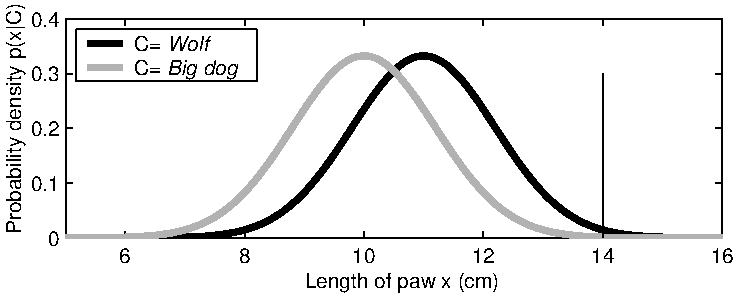
\includegraphics[width=11cm]{hatutus_likelihoods}
  observed length has been marked with a horizontal line
\item<+-> Likelihood of wolf is 0.92 (alternative being dog)
\end{list1}

\end{frame}

\begin{frame}
  
{\Large\color{navyblue} Example of decision making}

  \begin{list1}
  \item<+-> Helen assumes also that in her living area there are about one
    hundred times more free running dogs than wolves, that is {\em a
      priori} probability for wolf, before observation is 1\%.
  \item<+-> Likelihood and posterior
    \begin{center}\leavevmode
      \begin{tabular}{| l | c c |}
        \hline
        Animal &  Likelihood & Posterior probability \\
        \hline
        Wolf     &  0.92            & 0.10      \\
        Dog    &  0.08        & 0.90    \\
        \hline
      \end{tabular}
    \end{center}
  \item<+-> Posterior probability of wolf is 10\%
  \end{list1}

\end{frame}

\begin{frame}

{\Large\color{navyblue} Example of decision making}

  \begin{list1}
  \item<+-> Helen has to make decision whether to go pick mushrooms
  \item<+-> If she doesn't go to pick mushrooms utility is zero
  \item<+-> Helen assigns positive utility 1 for getting fresh mushrooms
  \item<+-> Helen assigns negative utility -1000 for a event that she goes to the forest and wolf attacks (for some reason Helen assumes that wolf will always attack)\\
    \vspace{0.5\baselineskip}
    \uncover<+->{
    \begin{minipage}[t]{58mm}
      \small
      \begin{tabular}{| l | c c |}
        \hline
        & \multicolumn{2}{ c |}{Animal} \\
        Decision ${\color{set12}d}$           & Wolf & Dog \\
        \hline
        Stay home             & 0    & 0              \\
        Go to the forest      & -1000 & 1      \\
        \hline
      \end{tabular}\\
      {Utility matrix ${\color{set13}U}({\color{set11}x})$}
    \end{minipage}
    }
    ~\\
    \vspace{0.5\baselineskip}
    \uncover<+->{
    \begin{minipage}[t]{58mm}
      \small
      \begin{tabular}{| l | c | }
        \hline
        & Expected utility \\
        Action $d$        &  $\E[{\color{set13}U}({\color{set11}x})\mid{\color{set12}d}]$ \\
        \hline
        Stay home         &  0       \\
        Go to the forest  &  -100+0.9     \\
        \hline
      \end{tabular}\\
      {Utilities for different actions}
    \end{minipage}
}
  \end{list1}

\end{frame}

\begin{frame}{Example of decision making}

  \begin{list1}
  \item<+-> Maximum likelihood decision would be to assume that there is a wolf
  \item<+-> Maximum posterior decision would be to assume that there is a dog
  \item<+-> Maximum utility decision is to stay home, even if it is more likely that the animal is dog
  \item<+-> Example illustrates that the uncertainties (probabilities)
    related to all consequences need to be carried on until final
    decision making
  \end{list1}

\end{frame}


% \begin{frame}

% {\Large\color{navyblue} Example of decision making: several choices}

% \begin{list1}
%   \item Prof. Gelman has a jar of quarters
%     \begin{list2}
%     \item he first drew a line on the side of the jar and then
%       filled the jar up to the line, and so the number coins was not
%       chosen beforehand
%     \item Prof. Gelman does not know the number of coins in the jar
%     \item<2-> Prof. Gelman gives the class a chance to win the coins if
%       they guess the number of coins correctly (someone else has
%       counted the coins without telling Gelman)
%     \item<2-> How should the students make the decision?
%     \end{list2}
% \end{list1}

% \end{frame}

\begin{frame}{Example of decision making: several choices}

\begin{list1}
\item You decide to earn money by selling a seasonal product
  \begin{list2}
  \item You pay 7€ per each, and sell them 10€ each
  \item You need to decide how many ($N$) items to buy
  \item<2-> You ask your friends how many they used to sell and estimate a
    distribution for how many you might sell
  \end{list2}
\end{list1}
\uncover<2>{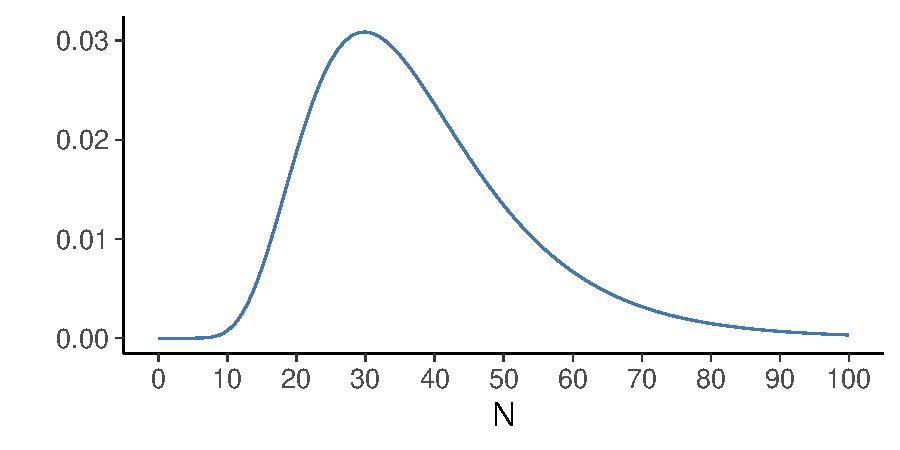
\includegraphics[width=9.5cm]{sales_dist1.pdf}}

\end{frame}

\begin{frame}{Example of decision making: several choices}

  {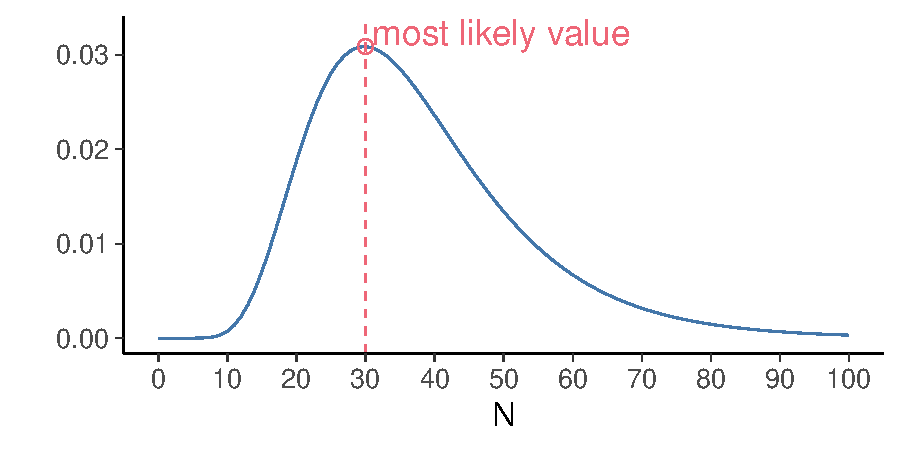
\includegraphics[width=9cm]{sales_dist2.pdf}}\\
  \only<2>{\vspace{-0.5\baselineskip}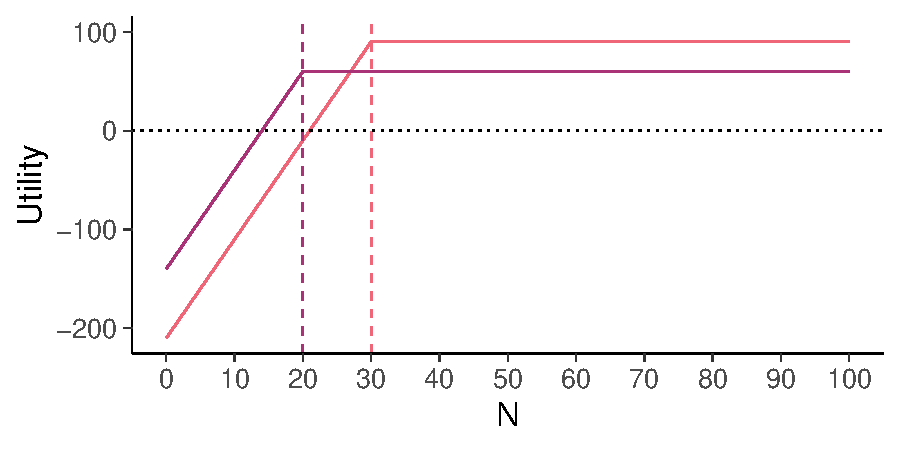
\includegraphics[width=9cm]{sales_utility_20_30.pdf}}
  \only<3>{\vspace{-0.5\baselineskip}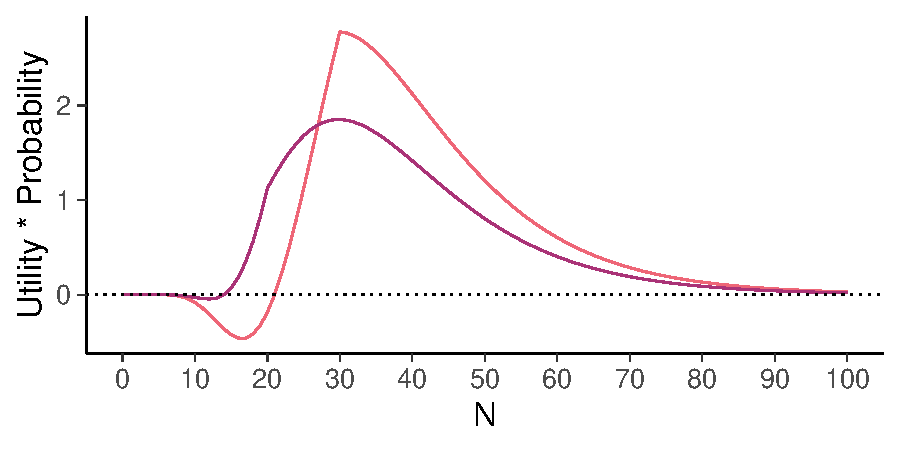
\includegraphics[width=9cm]{sales_utilprob_20_30.pdf}}
  \only<4>{\vspace{-0.5\baselineskip}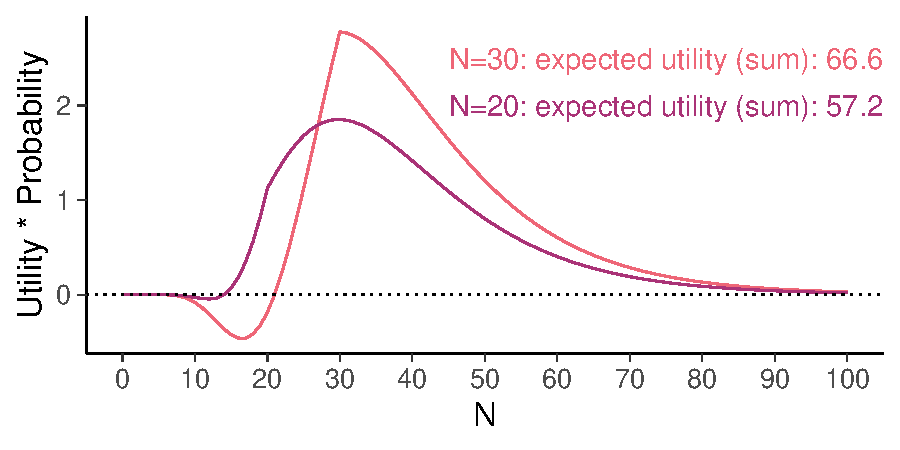
\includegraphics[width=9cm]{sales_utilprob_exputil_20_30.pdf}}
  \only<5>{\vspace{-0.5\baselineskip}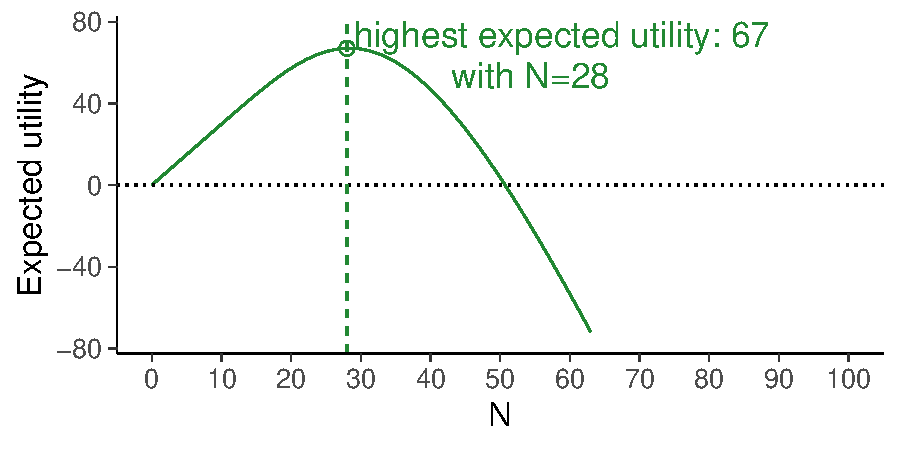
\includegraphics[width=9cm]{sales_exputil.pdf}}
  
\end{frame}  

\begin{frame}{Decision making in sales}

  \begin{list1}
    \item Common task in commerce and restaurants
  \end{list1}
  
\end{frame}  


\begin{frame}{Challenges in decision making}

  \begin{list1}
  \item Actual utility functions are rarely linear
    \begin{list2}
    \item<2-> the expected utility is 5€ for\\
      a) 100\% of receiving 5€\\
      b) 50\% of losing 1M€ and 50\% of winning 1M€ + 10€
    \item<3-> most gambling has negative expected utility\\
      (but the excitement of the game may have positive utility)
    \end{list2}
  \item<4-> What is the cost of human life?
  \item<5-> Multiple parties having different utilities
  \end{list1}
  
\end{frame}

\begin{frame}{Model selection as decision problem}

  \begin{list1}
  \item Choose the model that maximizes the expected utility of using
    the model to make predictions / decisions in the future
  \end{list1}

\end{frame}

\begin{frame}{Multi-stage decision making (Section 9.3)}

  \vspace{-0.3\baselineskip}
  \begin{list1}
  \item<+-> 95 year old has a tumor that is malignant with 90\% prob
  \item<+-> Based on statistics
    \begin{list2}
    \item<.-> expected lifetime is 34.8 months if no cancer
    \item<+-> expected lifetime is 16.7 months if cancer and radiation therapy is used
    \item<+-> expected lifetime is 20.3 months if cancer and surgery, but the probability of dying in surgery is 35\% (for 95 year old)
    \item<+-> expected lifetime is 5.6 months if cancer and no treatment
    \end{list2}
  \item<+-> Which treatment to choose?
    \begin{list2}
    \item<.-> quality adjusted life time
    \item<.-> 1 month is subtracted for the time spent in treatments
    \end{list2}
   \item<+-> Quality adjusted life time
    \begin{list2}
    \item<.-> See the book for the multi-stage decision making
   %  \item<.-> Radiotherapy: 0.9*16.7 + 0.1*34.8 - 1 = 17.5mo
   % \item<+-> Surgery: 0.35*0 + 0.65*(0.9*20.3 + 0.1*34.8 - 1) = 13.5mo
   %  \item<+-> No treatment: 0.9*5.6 + 0.1*34.8 = 8.5mo
    \end{list2}
  % \item<+-> See the book for continuation of the example with
  %   additional test for cancer
\end{list1}

\end{frame}

\begin{frame}{Design of experiment}

  \begin{list1}
  \item Which experiment would give most additional information
    \begin{list2}
    \item decide values $x_{n+1}$ for the next experiment
    \item which values of $x_{n+1}$ would reduce the posterior
      uncertainty or increase the expected utility most
    \end{list2}
  \item<2-> Example 1
    \begin{list2}
      \item biopsy in the cancer example
    \end{list2}
  \item<3-> Example 2
    \begin{list2}
    \item imagine that in bioassay the posterior uncertainty of LD50 is too large
    \item which dose should be used in the next experiment to reduce
      the variance of LD50 as much as possible ?
      \begin{list3}
        \item this way fewer experiments need to be made (and fewer animals need to be killed)
      \end{list3}
    \end{list2}
  \item<4-> Example 3
    \begin{list2}
      \item optimal paper helicopter wing length
    \end{list2}
  \end{list1}
\end{frame}

\begin{frame}{Bayesian optimization}

  \begin{list1}
  \item Design of experiment
  \item Used to optimize, for example,
    \begin{list2}
    \item machine learning / deep learning model structures,
      regularization, and learning algorithm parameters
    \item material science
    \item engines
    \item drug testing
    \item part of Bayesian inference for stochastic simulators
    \end{list2}
  \end{list1}

\end{frame}

\begin{frame}{Bayesian optimization of wing length}

\only<1>{Start with a small number of experiments\\
  \hspace{-8mm}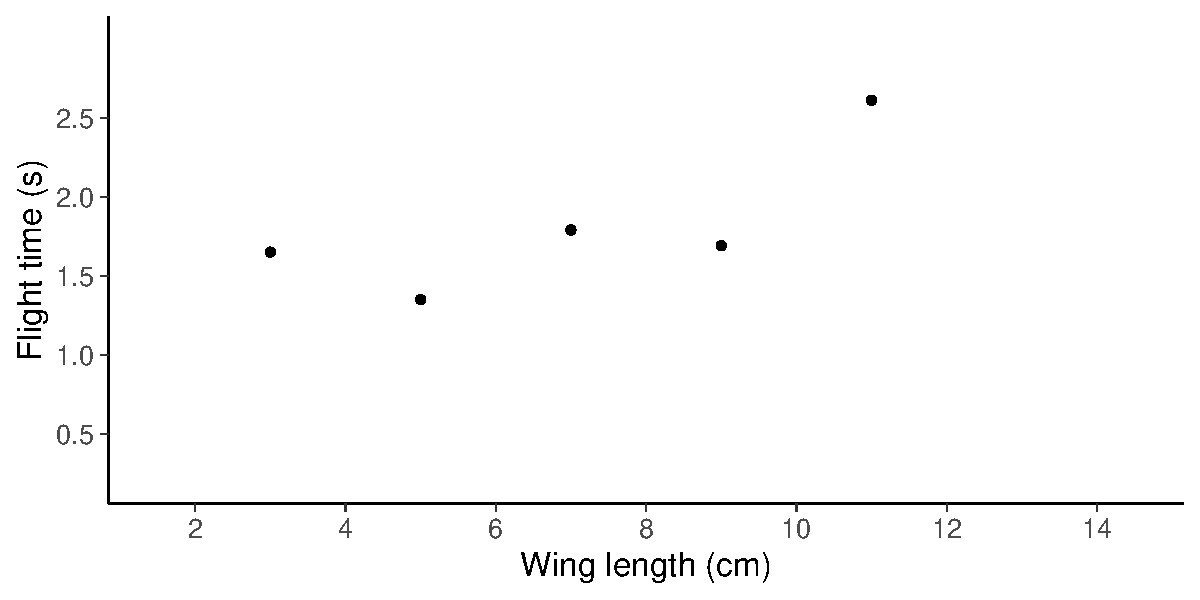
\includegraphics[width=11.5cm]{helicopter_bo_initial_data.pdf}\\}
\only<2>{Gaussian process model\\
\hspace{-8mm}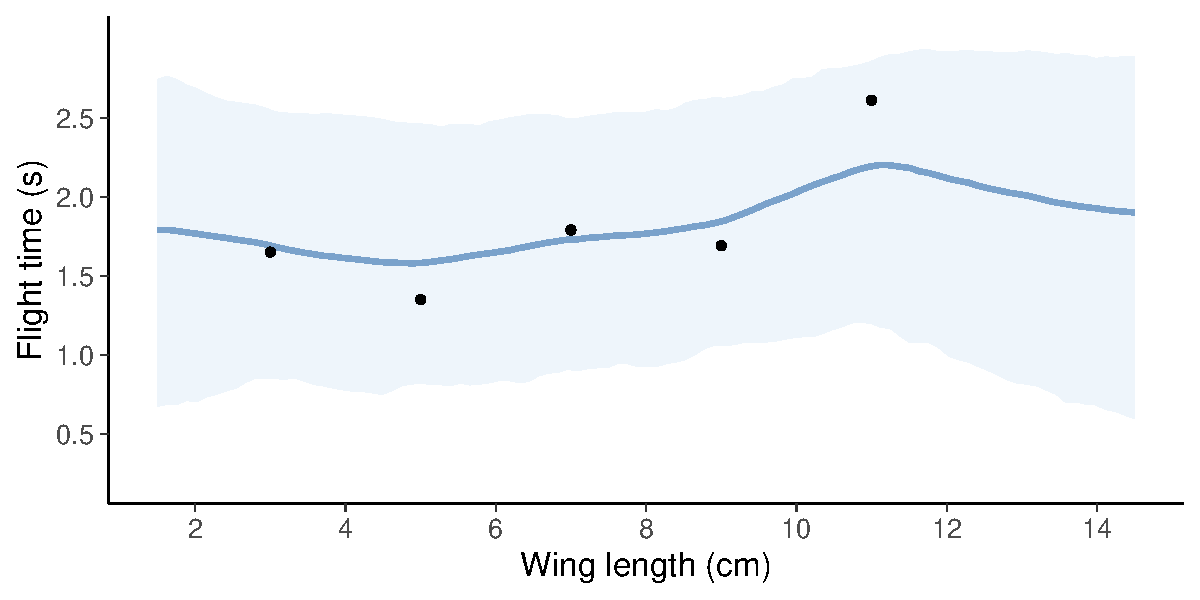
\includegraphics[width=11.5cm]{helicopter_bo_initial_fit.pdf}\\}
\only<3-4>{Gaussian process model -- posterior draws\\
  \hspace{-8mm}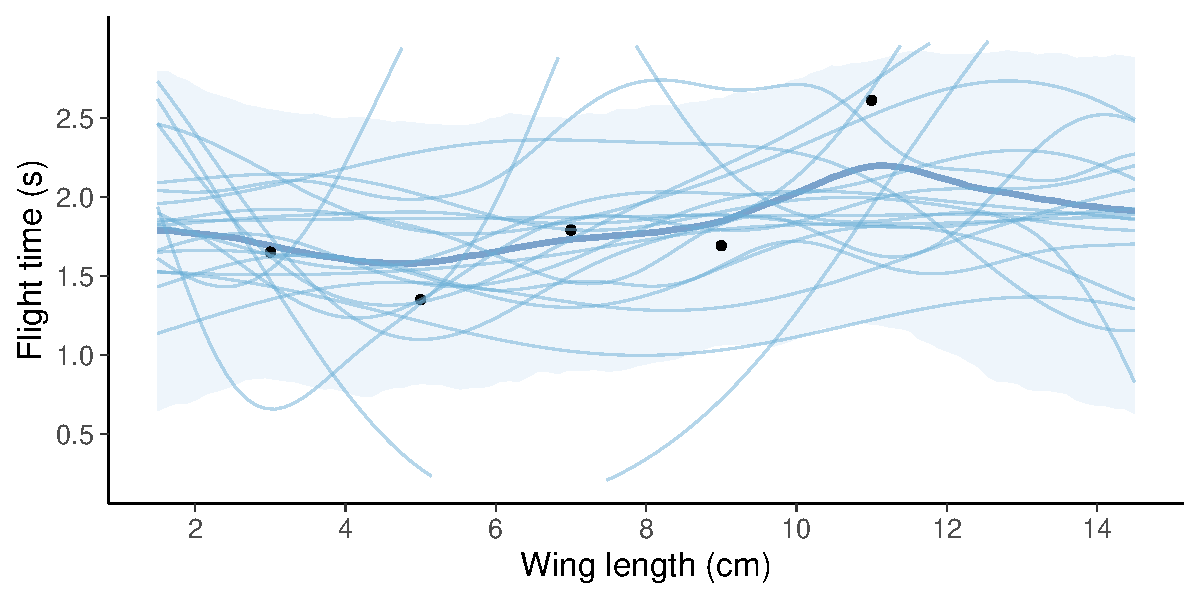
\includegraphics[width=11.5cm]{helicopter_bo_initial_fit_draws.pdf}\\}
\only<5>{Gaussian process model -- Thompson sampling\\
  \hspace{-8mm}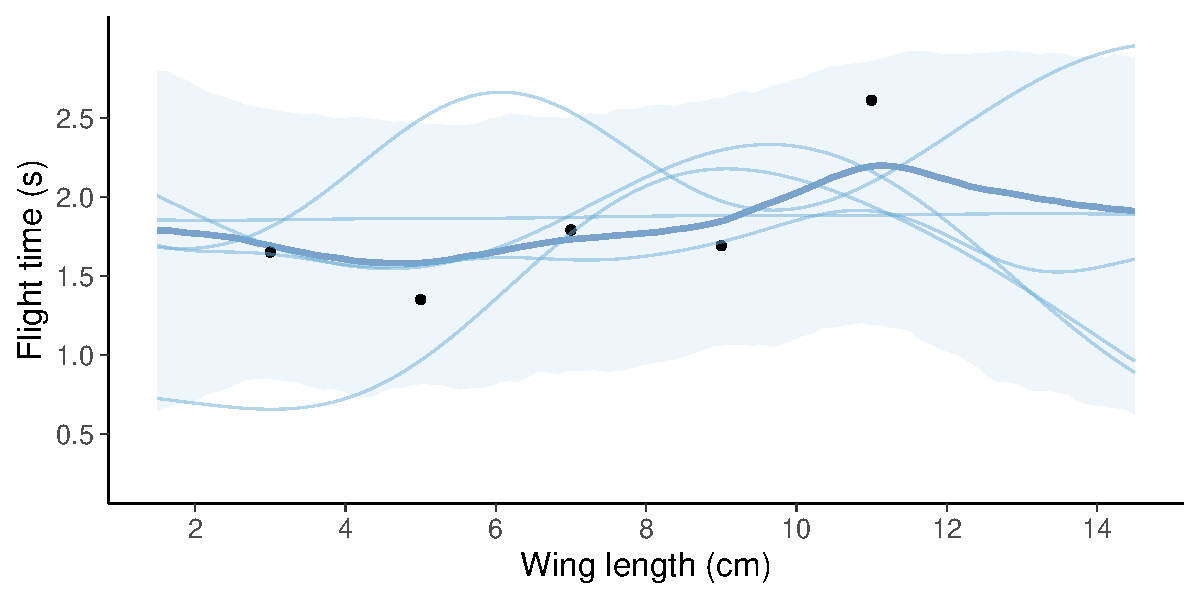
\includegraphics[width=11.5cm]{helicopter_bo_a_1.pdf}\\}
\only<6>{Gaussian process model -- Thompson sampling\\
  \hspace{-8mm}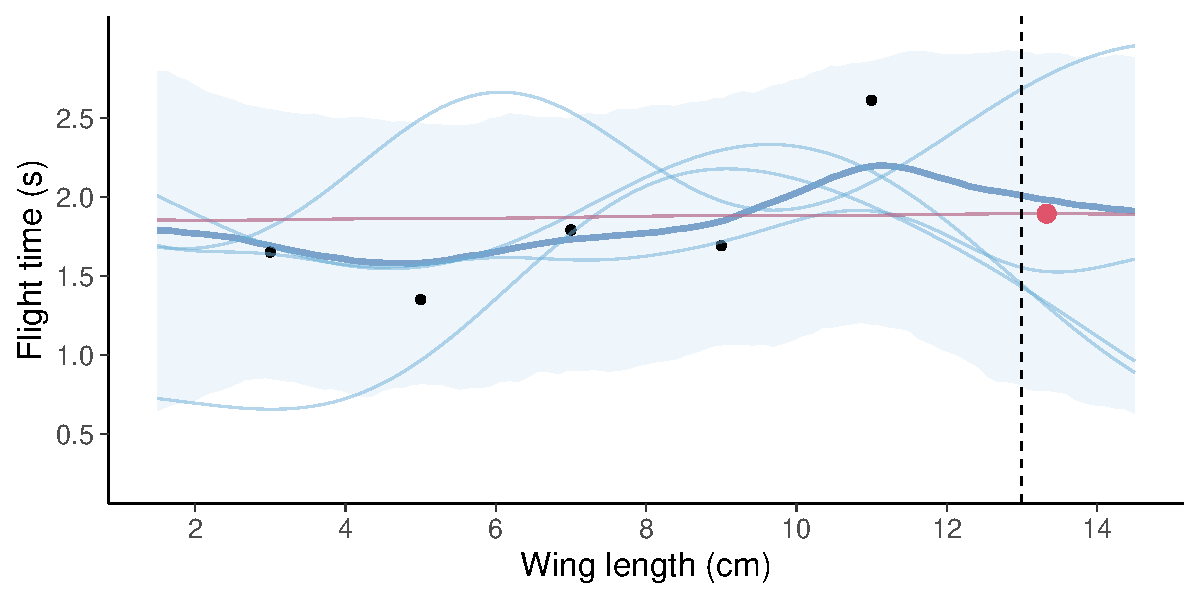
\includegraphics[width=11.5cm]{helicopter_bo_b_1.pdf}\\}

{\vspace{-0.5\baselineskip}}
\begin{list1}
  \item<4-> Thompson sampling:
    \begin{list2}
    \item pick one posterior draw (function)
    \item find the wing length corresponding to the max. of that draw
    \item make the next observation with that wing length
    \end{list2}
  \end{list1}
  
\end{frame}

\begin{frame}{Bayesian optimization of wing length}

  Gaussian process model -- Thompson sampling\\
\only<+>{\hspace{-8mm}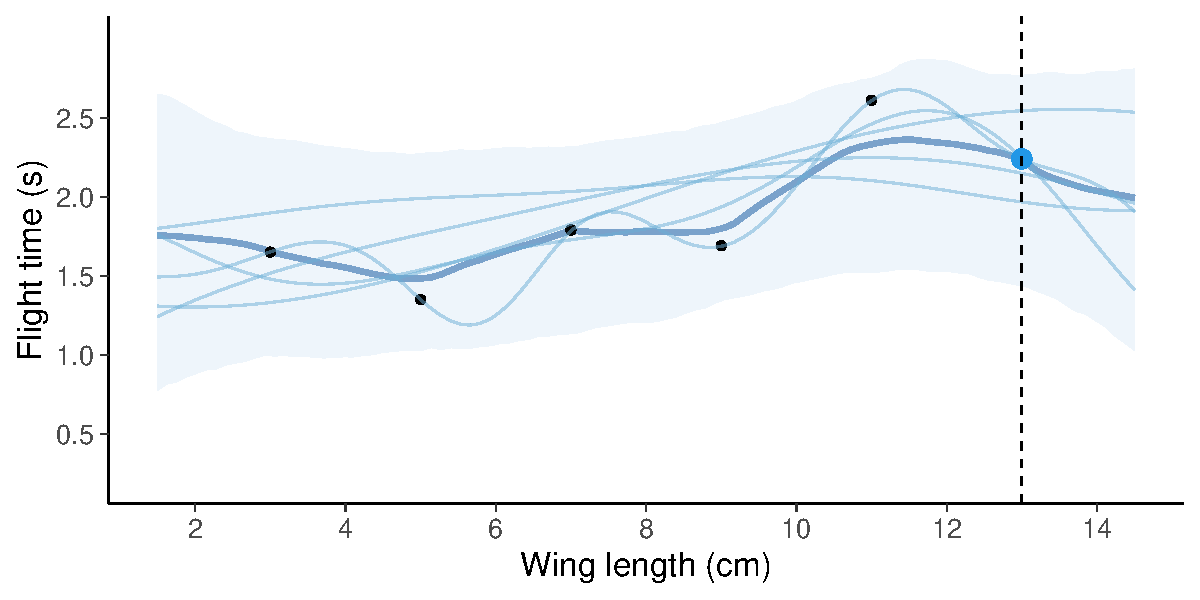
\includegraphics[width=11.5cm]{helicopter_bo_a_2.pdf}}
\only<+>{\hspace{-8mm}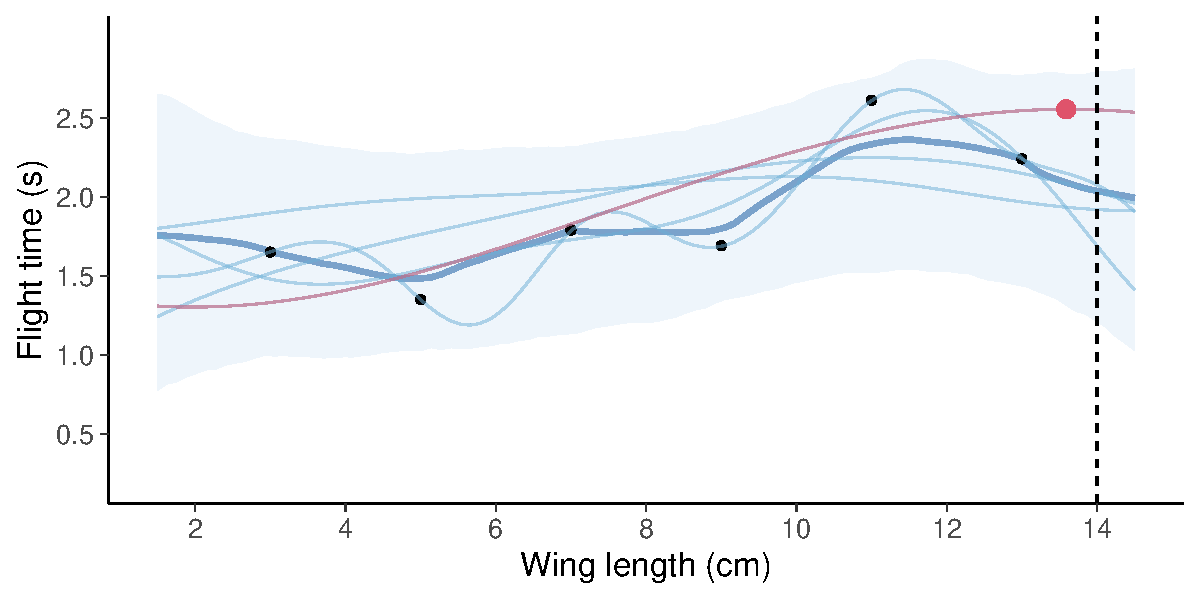
\includegraphics[width=11.5cm]{helicopter_bo_b_2.pdf}}
\only<+>{\hspace{-8mm}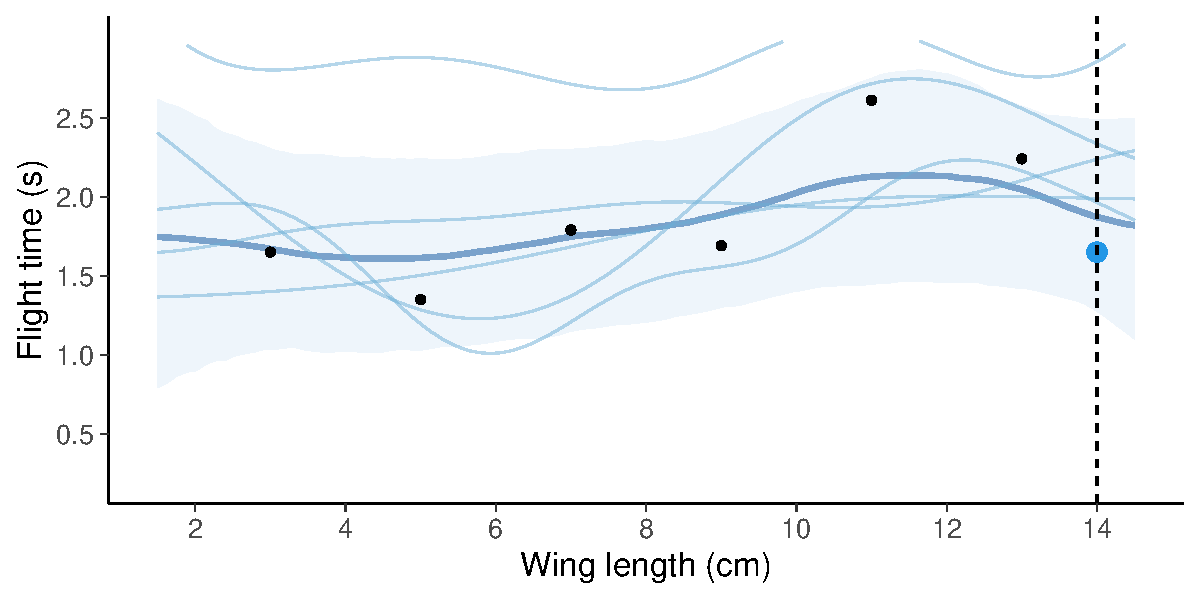
\includegraphics[width=11.5cm]{helicopter_bo_a_3.pdf}}
\only<+>{\hspace{-8mm}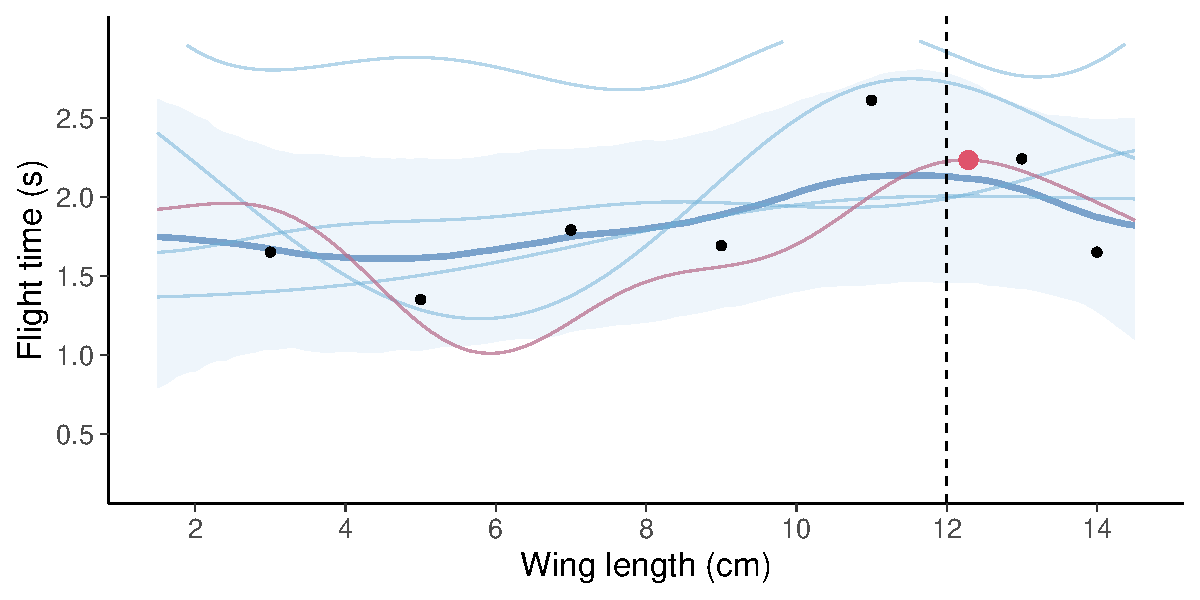
\includegraphics[width=11.5cm]{helicopter_bo_b_3.pdf}}
\only<+>{\hspace{-8mm}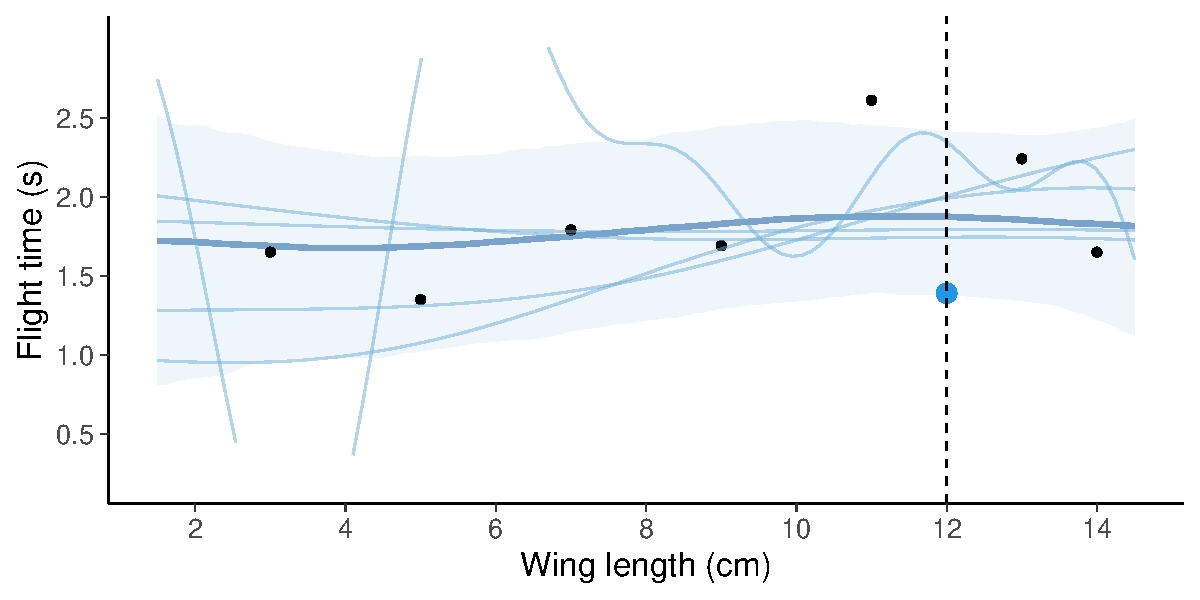
\includegraphics[width=11.5cm]{helicopter_bo_a_4.pdf}}
\only<+>{\hspace{-8mm}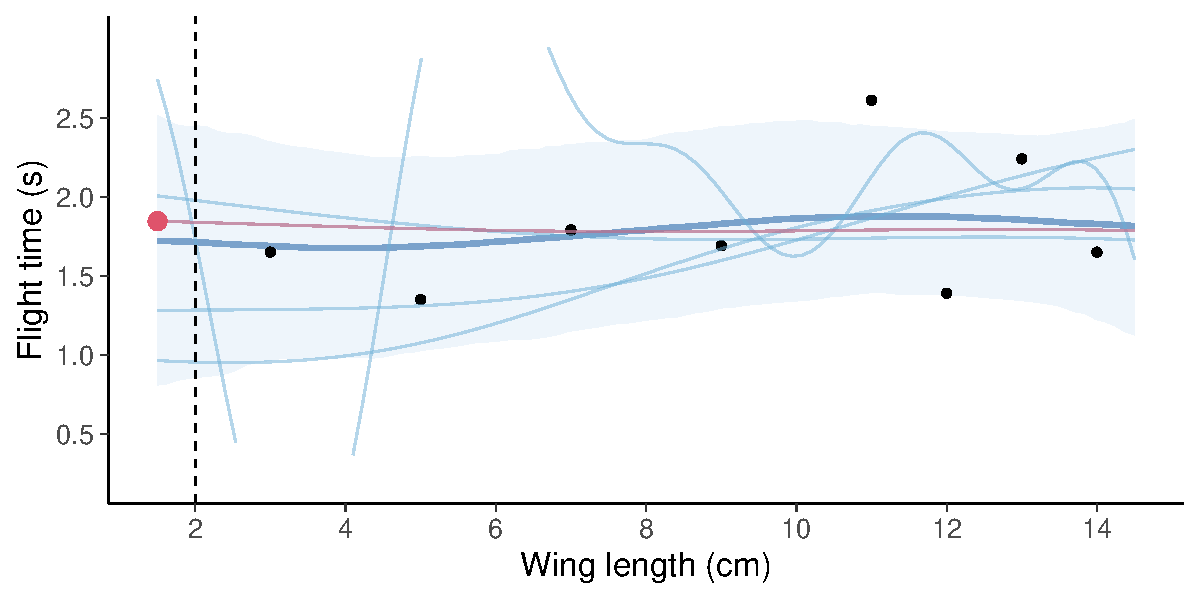
\includegraphics[width=11.5cm]{helicopter_bo_b_4.pdf}}
\only<+>{\hspace{-8mm}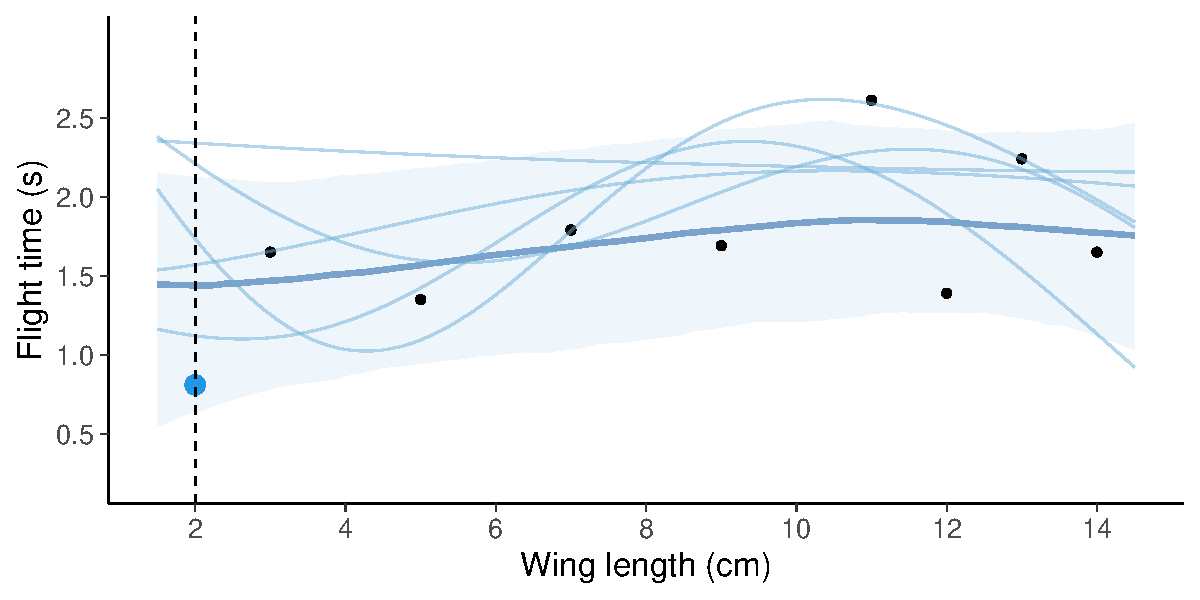
\includegraphics[width=11.5cm]{helicopter_bo_a_5.pdf}}
\only<+>{\hspace{-8mm}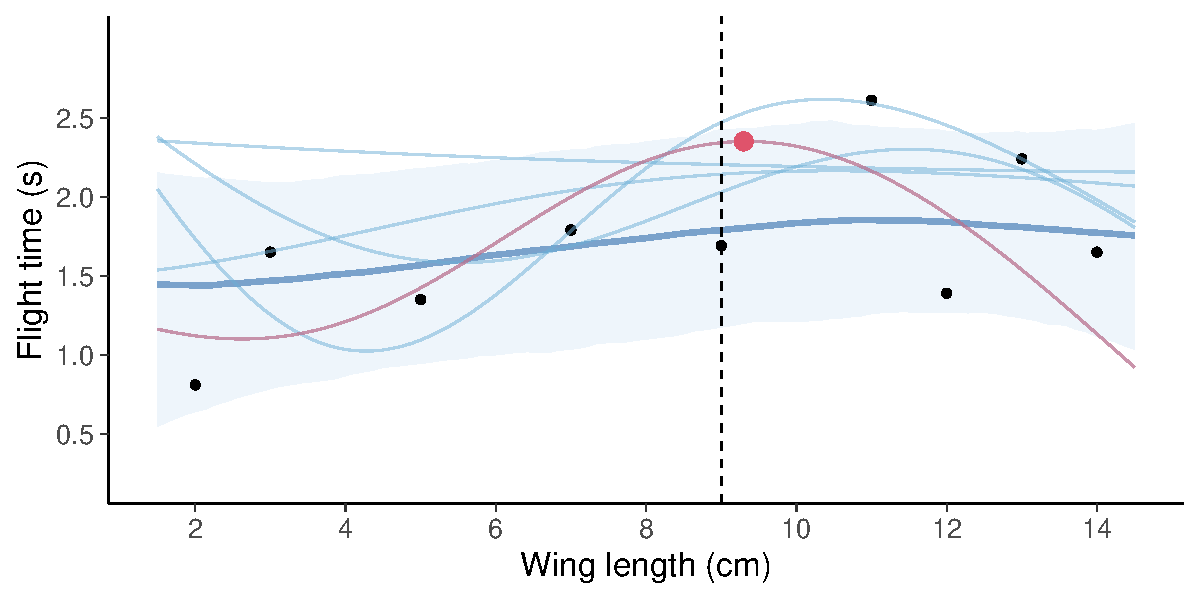
\includegraphics[width=11.5cm]{helicopter_bo_b_5.pdf}}
\only<+>{\hspace{-8mm}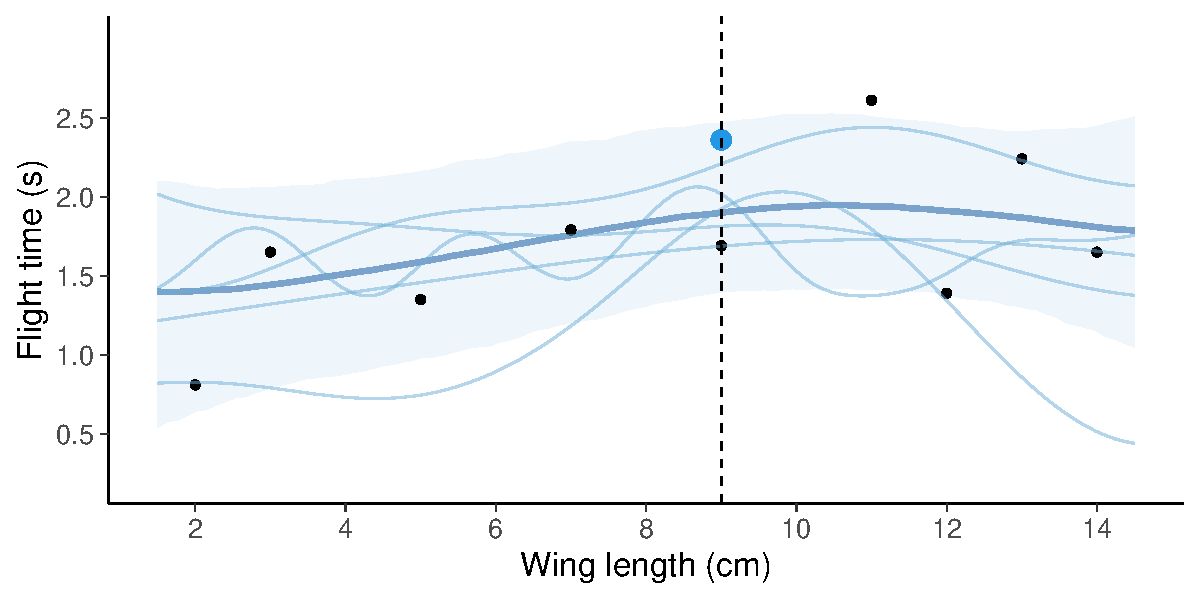
\includegraphics[width=11.5cm]{helicopter_bo_a_6.pdf}}
\only<+>{\hspace{-8mm}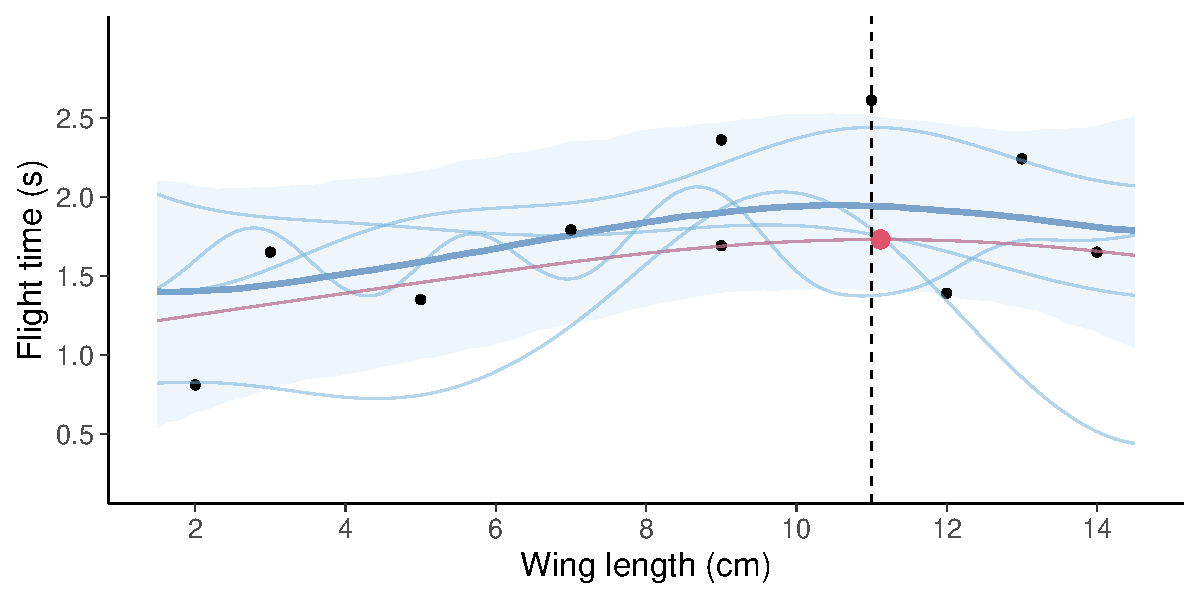
\includegraphics[width=11.5cm]{helicopter_bo_b_6.pdf}}
\only<+>{\hspace{-8mm}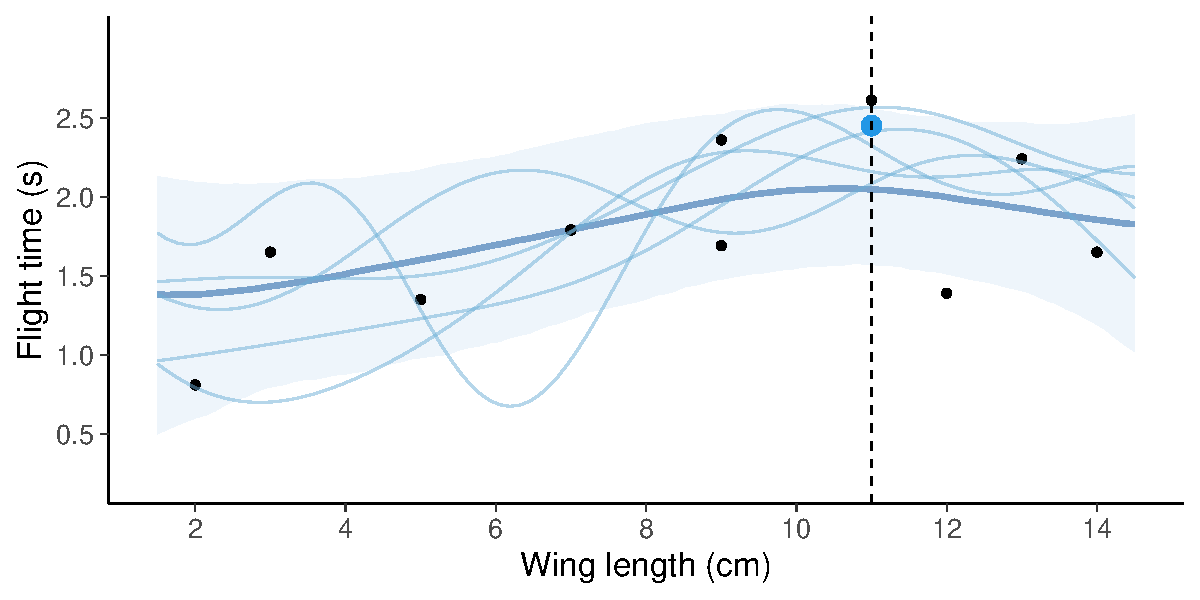
\includegraphics[width=11.5cm]{helicopter_bo_a_7.pdf}}
\only<+>{\hspace{-8mm}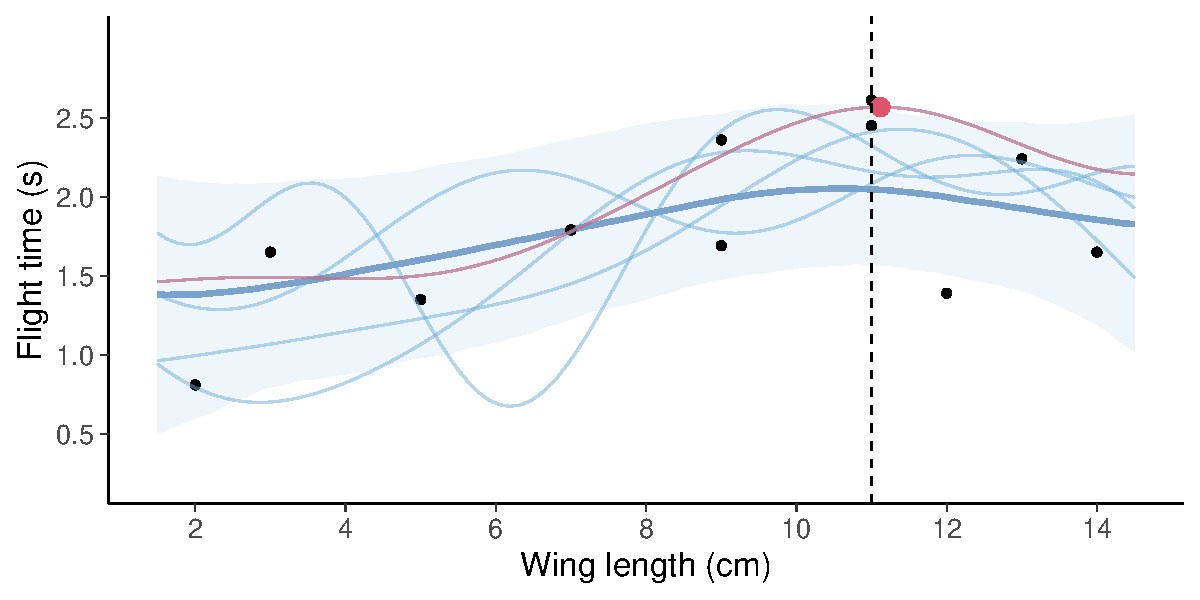
\includegraphics[width=11.5cm]{helicopter_bo_b_7.pdf}}
\only<+>{\hspace{-8mm}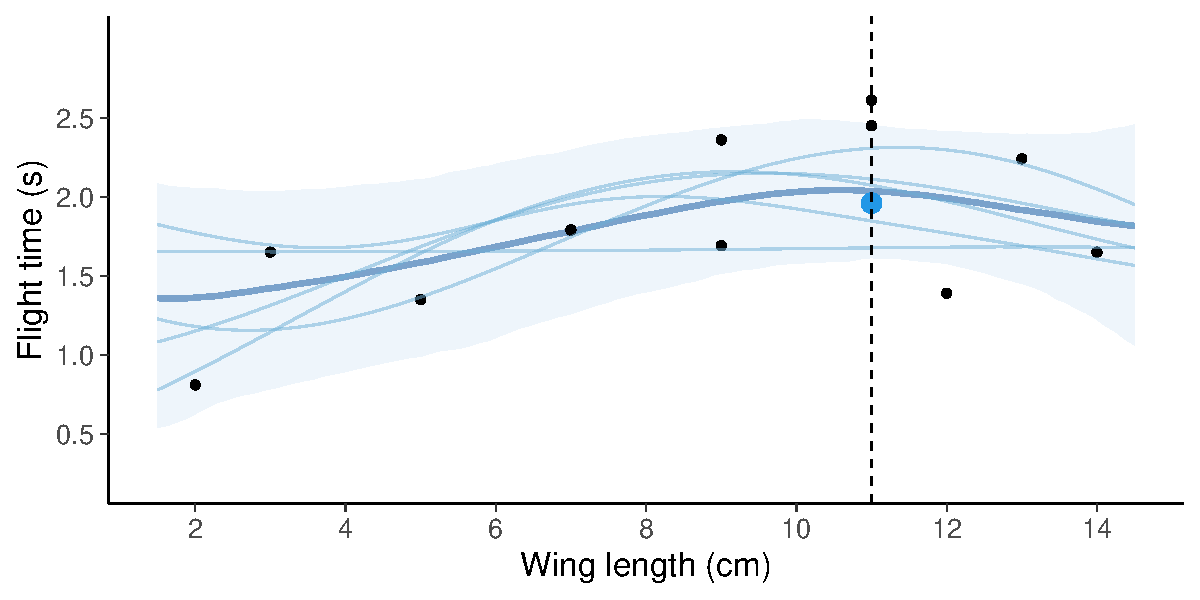
\includegraphics[width=11.5cm]{helicopter_bo_a_8.pdf}}
\only<+>{\hspace{-8mm}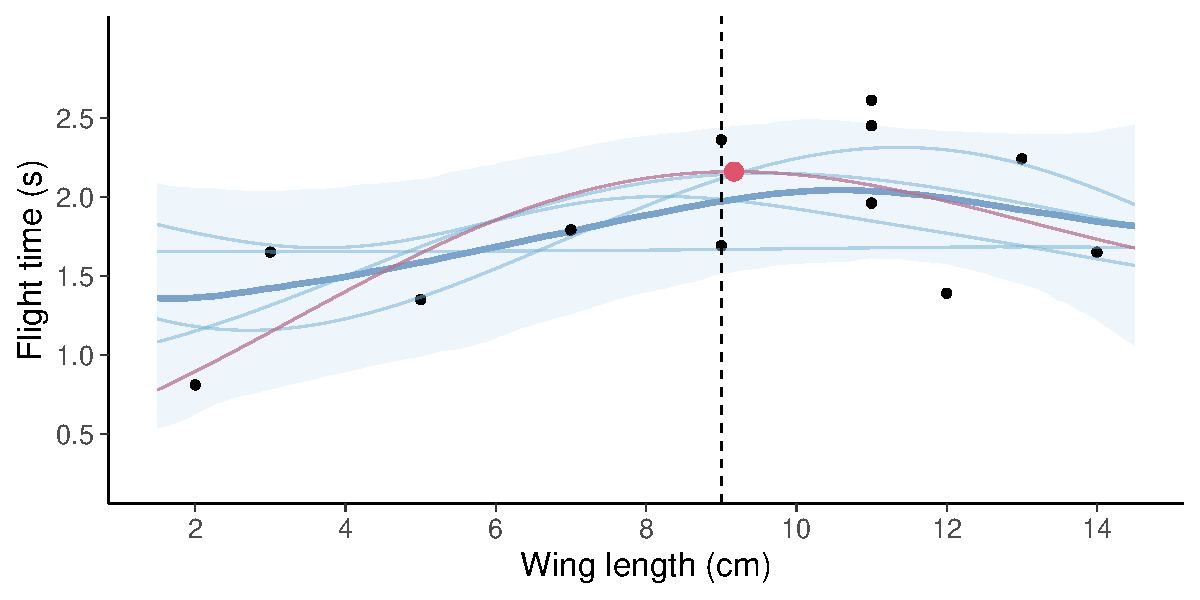
\includegraphics[width=11.5cm]{helicopter_bo_b_8.pdf}}
\only<+>{\hspace{-8mm}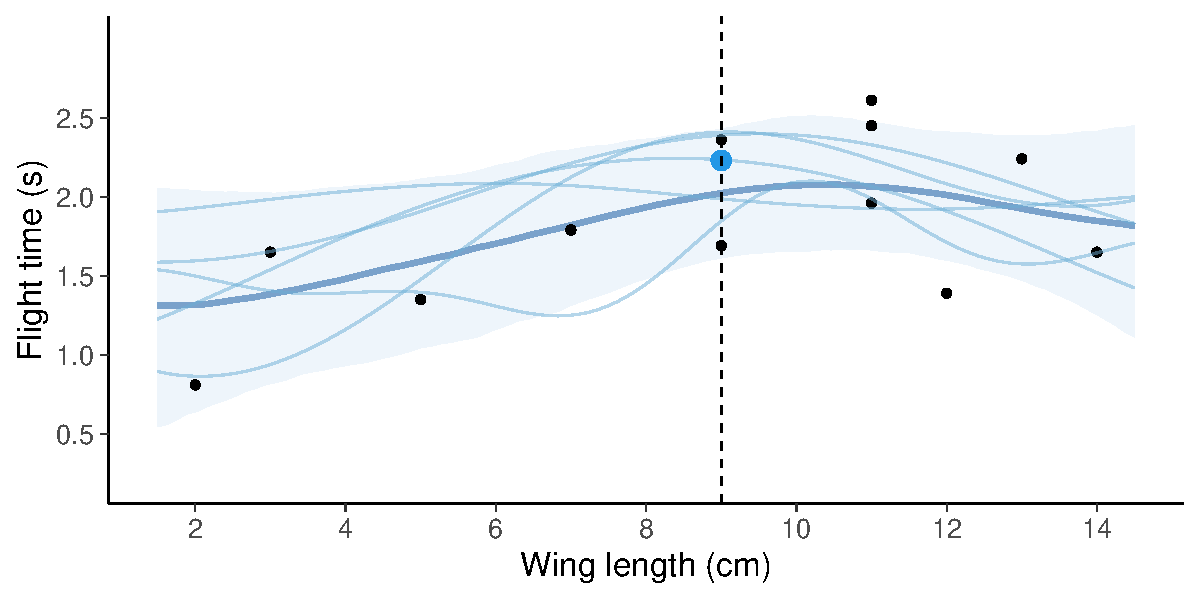
\includegraphics[width=11.5cm]{helicopter_bo_a_9.pdf}}
\only<+>{\hspace{-8mm}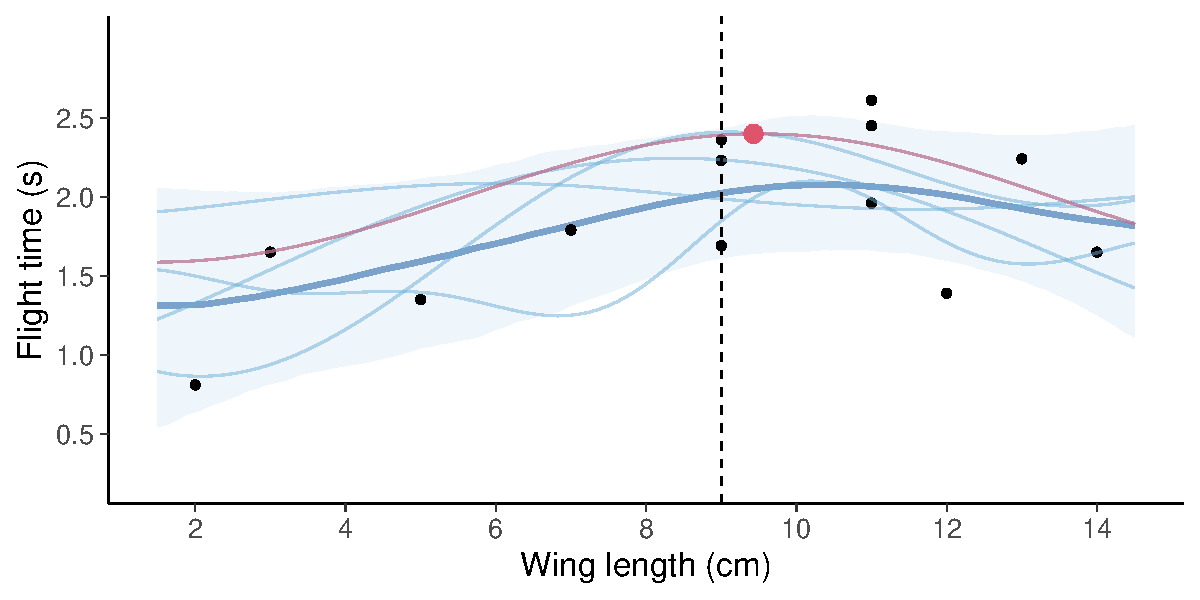
\includegraphics[width=11.5cm]{helicopter_bo_b_9.pdf}}
\only<+>{\hspace{-8mm}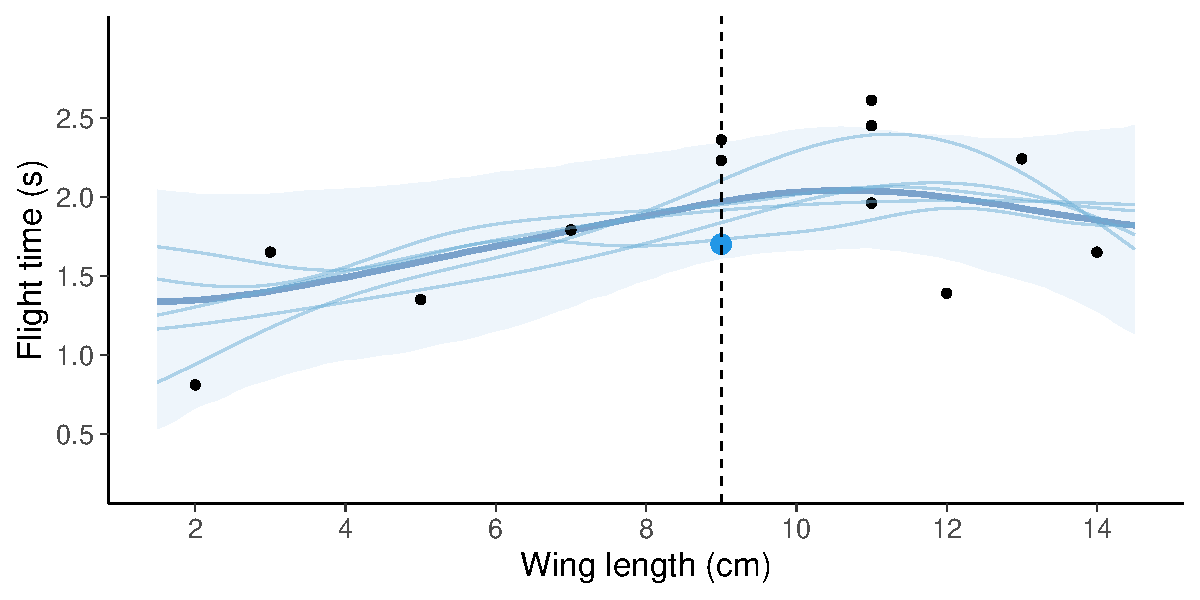
\includegraphics[width=11.5cm]{helicopter_bo_a_10.pdf}}
\only<+>{\hspace{-8mm}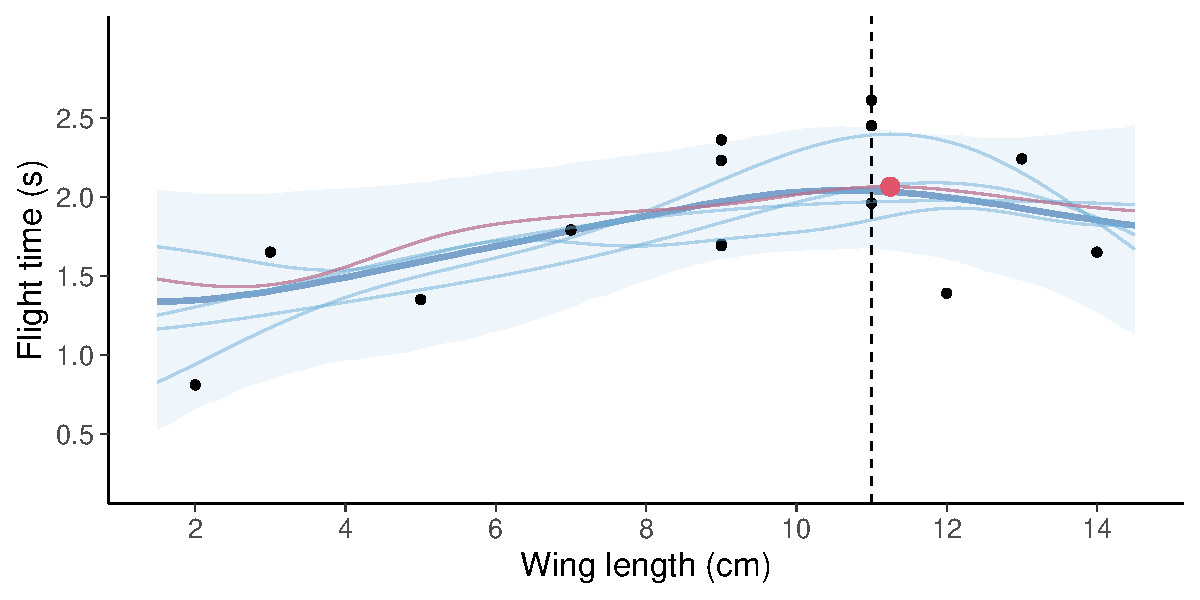
\includegraphics[width=11.5cm]{helicopter_bo_b_10.pdf}}
\only<+>{\hspace{-8mm}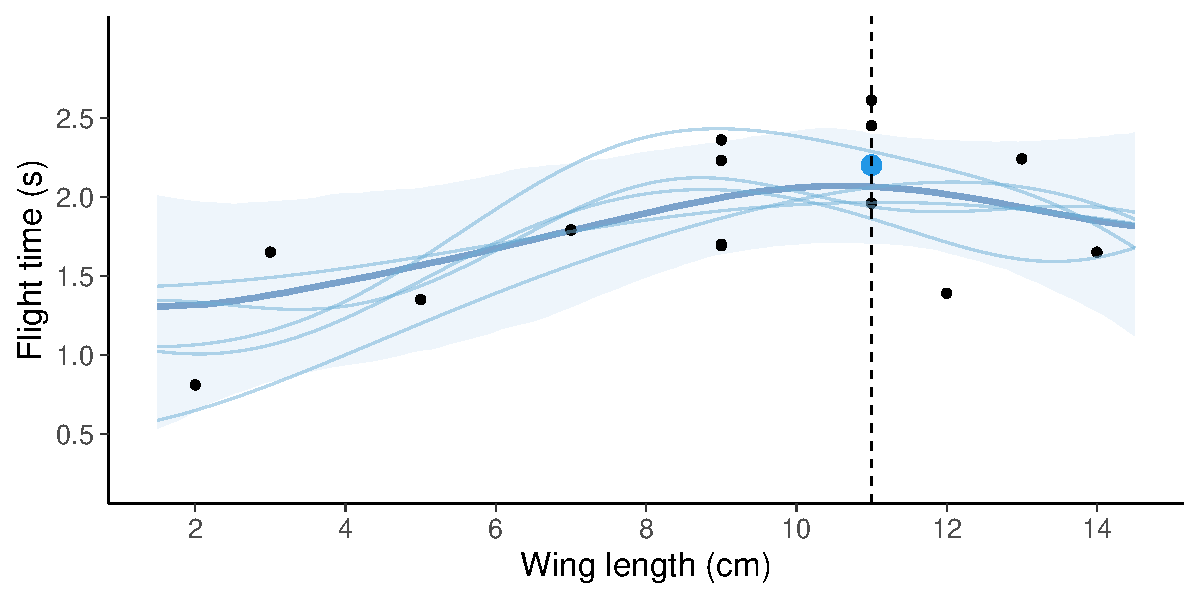
\includegraphics[width=11.5cm]{helicopter_bo_a_11.pdf}}
\only<+>{\hspace{-8mm}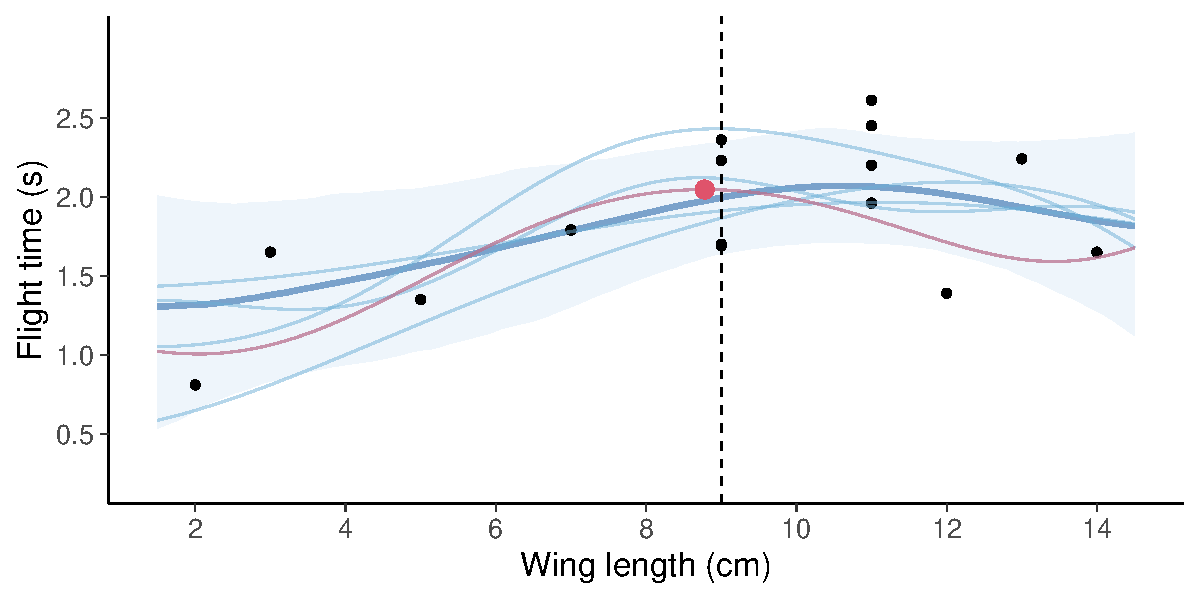
\includegraphics[width=11.5cm]{helicopter_bo_b_11.pdf}}
\only<+>{\hspace{-8mm}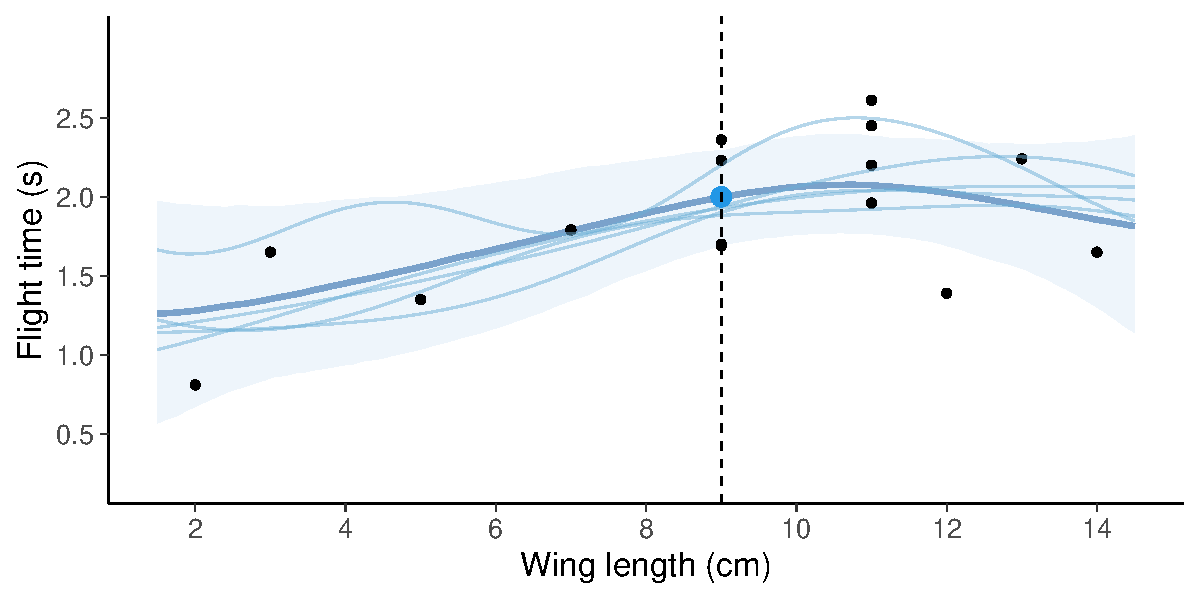
\includegraphics[width=11.5cm]{helicopter_bo_a_12.pdf}}
\only<+>{\hspace{-8mm}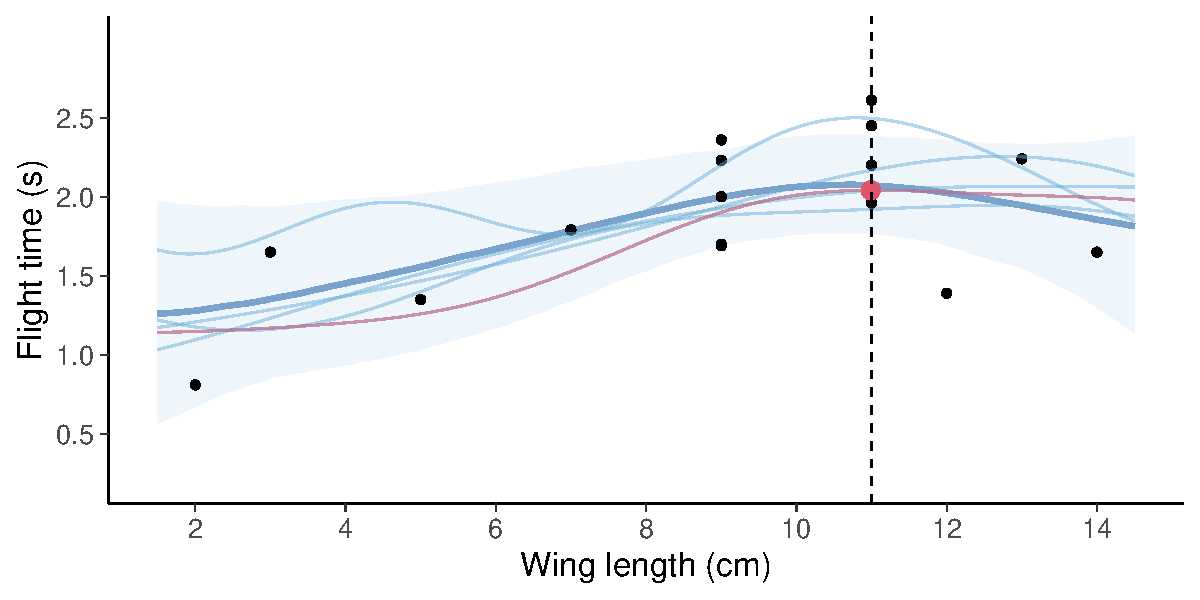
\includegraphics[width=11.5cm]{helicopter_bo_b_12.pdf}}
\only<+>{\hspace{-8mm}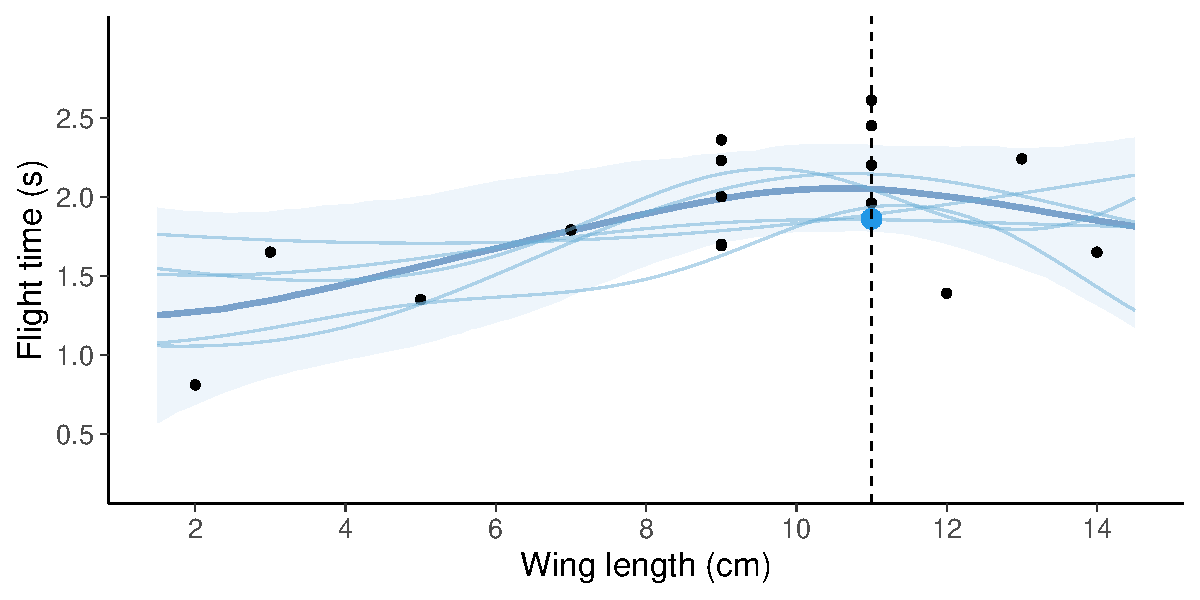
\includegraphics[width=11.5cm]{helicopter_bo_a_13.pdf}}
\only<+>{\hspace{-8mm}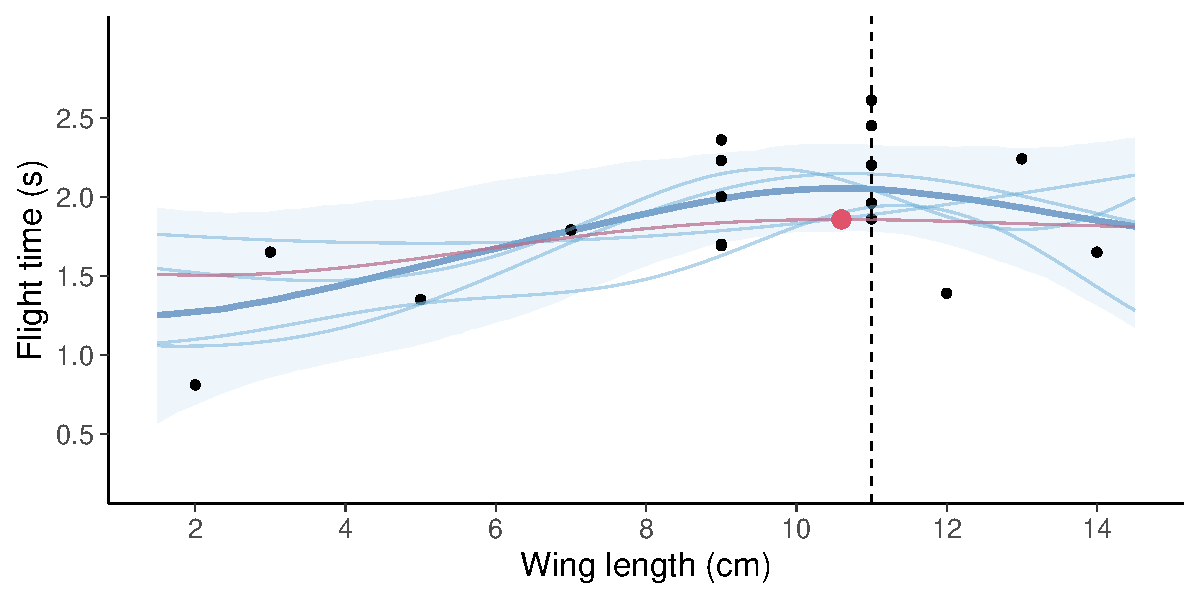
\includegraphics[width=11.5cm]{helicopter_bo_b_13.pdf}}
\only<+>{\hspace{-8mm}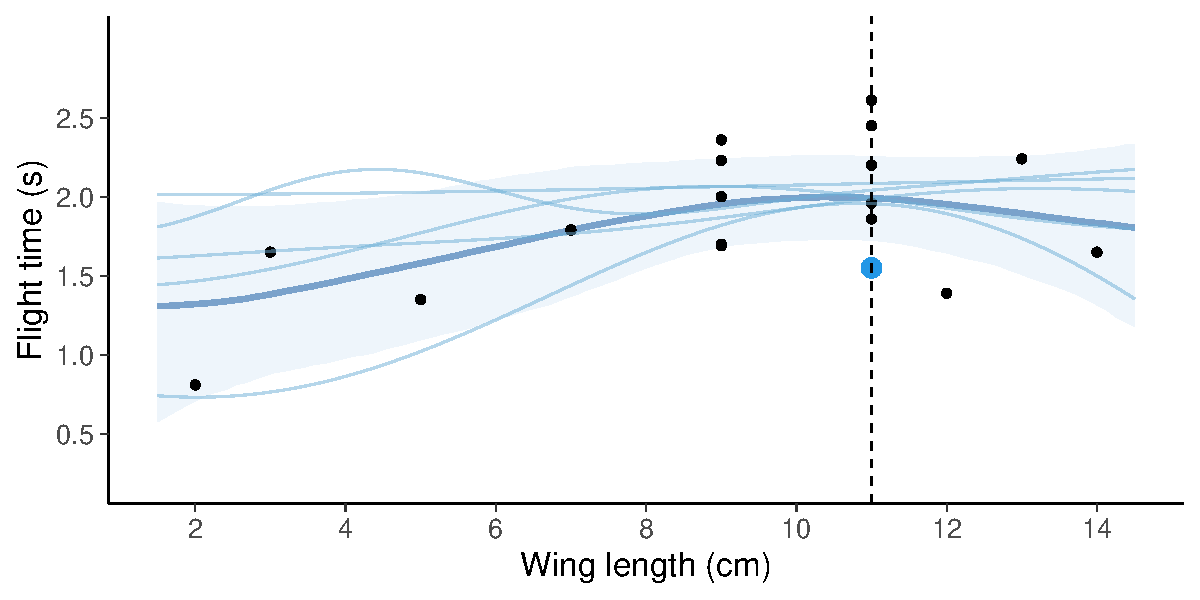
\includegraphics[width=11.5cm]{helicopter_bo_a_14.pdf}}
\only<+>{\hspace{-8mm}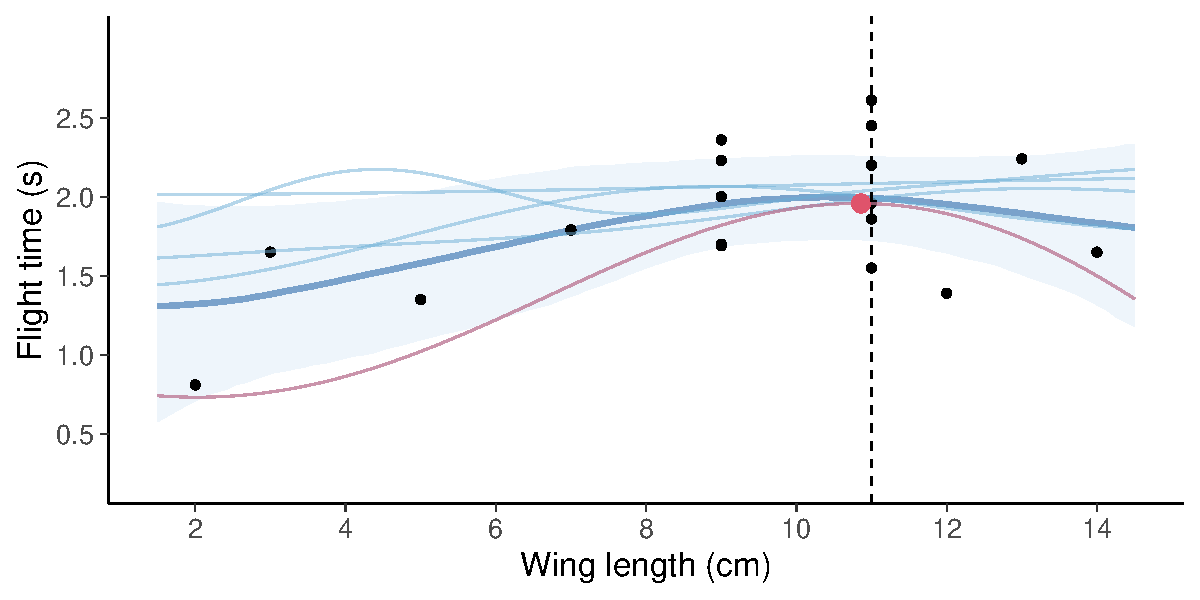
\includegraphics[width=11.5cm]{helicopter_bo_b_14.pdf}}
\only<+>{\hspace{-8mm}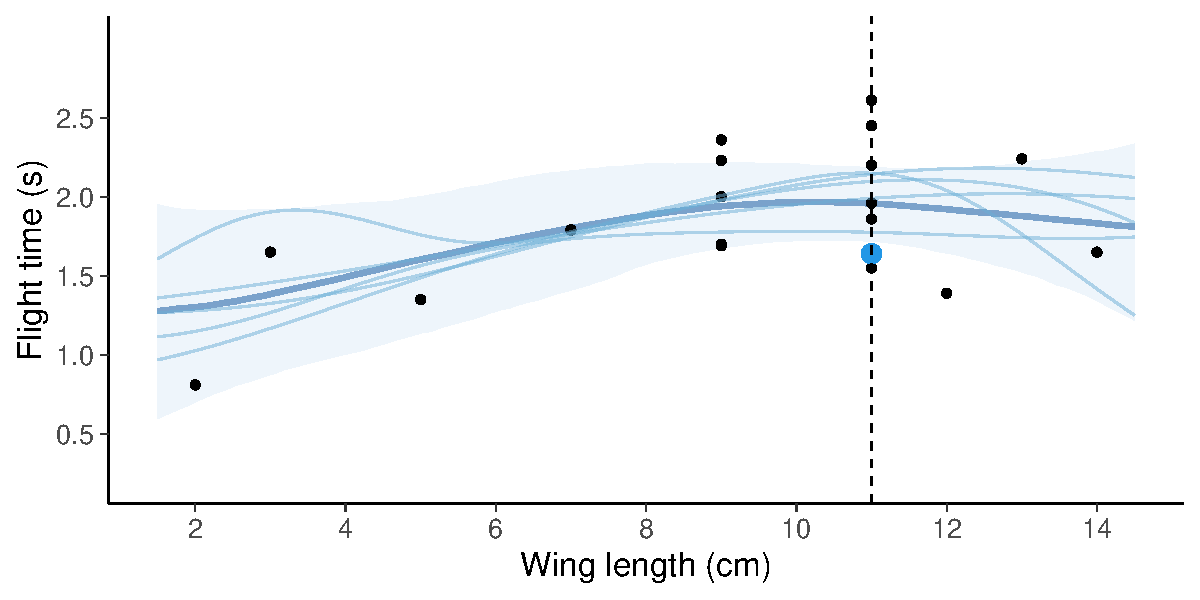
\includegraphics[width=11.5cm]{helicopter_bo_a_15.pdf}}
\only<+>{\hspace{-8mm}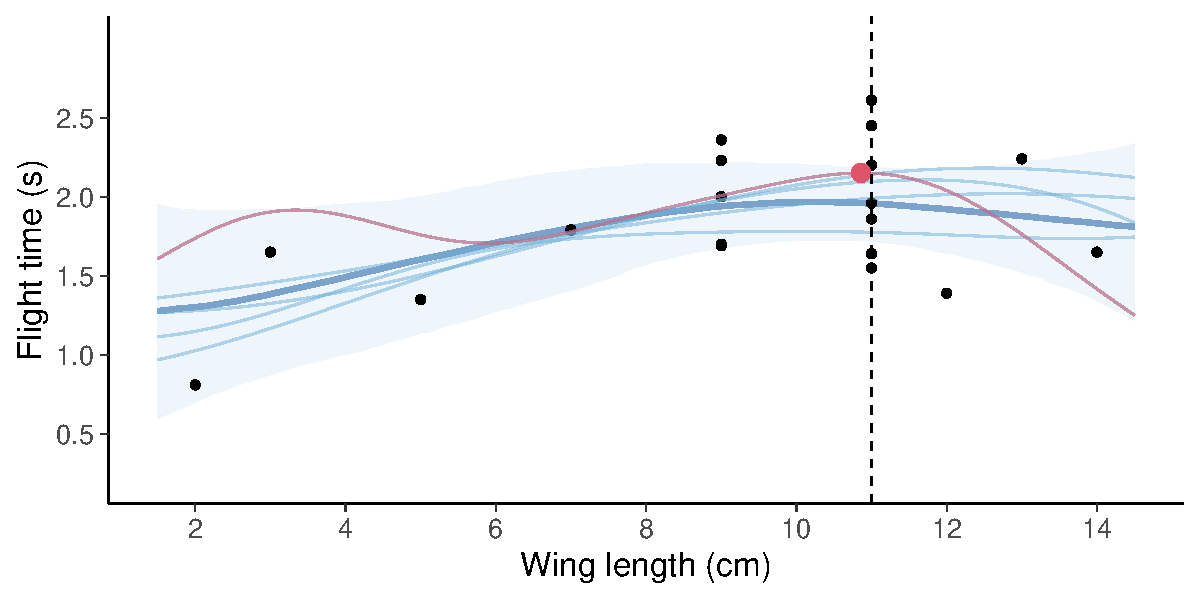
\includegraphics[width=11.5cm]{helicopter_bo_b_15.pdf}}
\only<+>{\hspace{-8mm}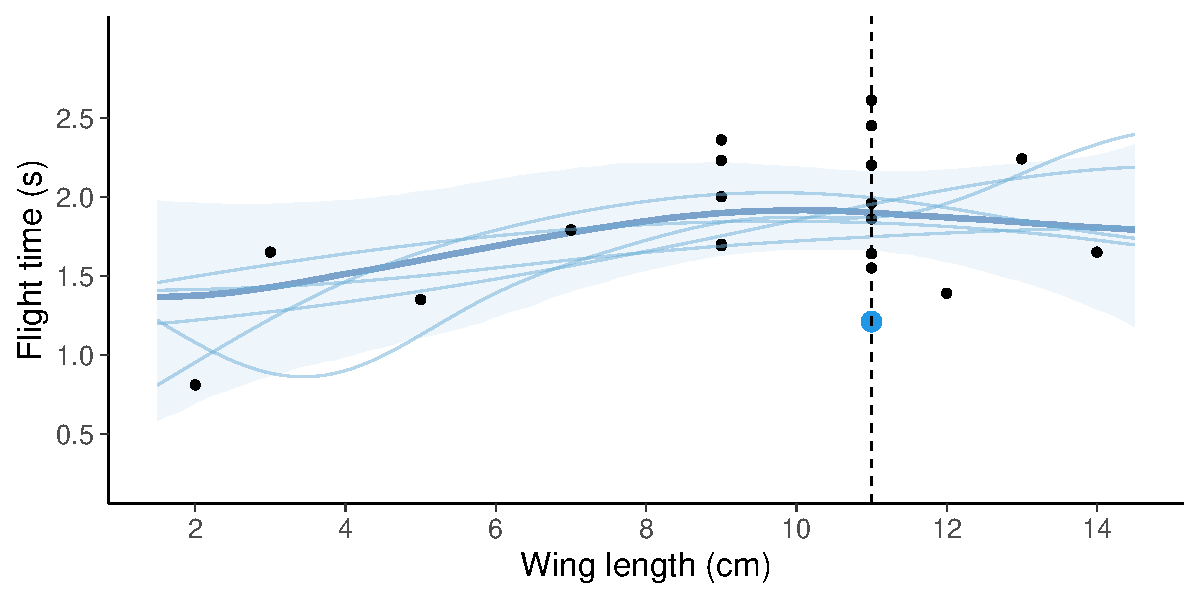
\includegraphics[width=11.5cm]{helicopter_bo_a_16.pdf}}
\only<+>{\hspace{-8mm}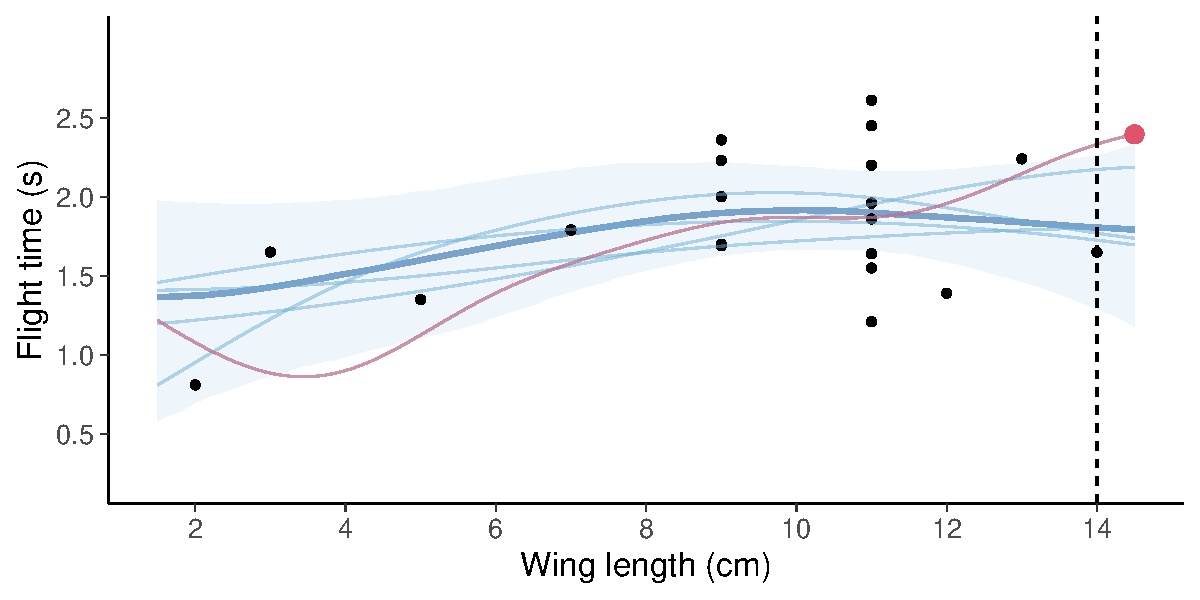
\includegraphics[width=11.5cm]{helicopter_bo_b_16.pdf}}
\only<+>{\hspace{-8mm}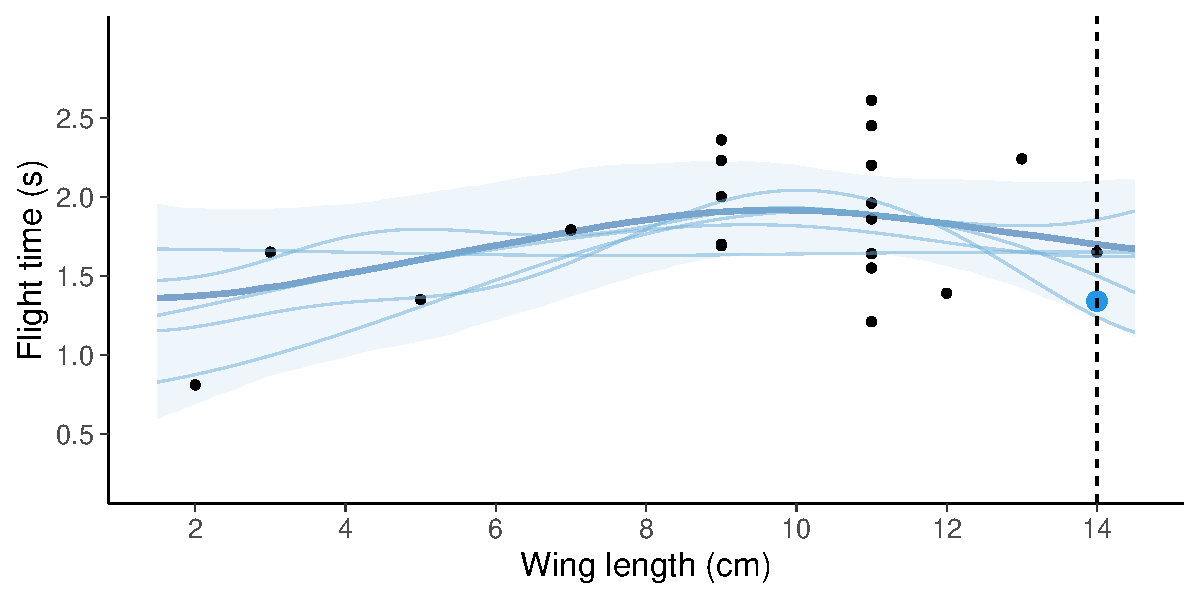
\includegraphics[width=11.5cm]{helicopter_bo_a_17.pdf}}
\only<+>{\hspace{-8mm}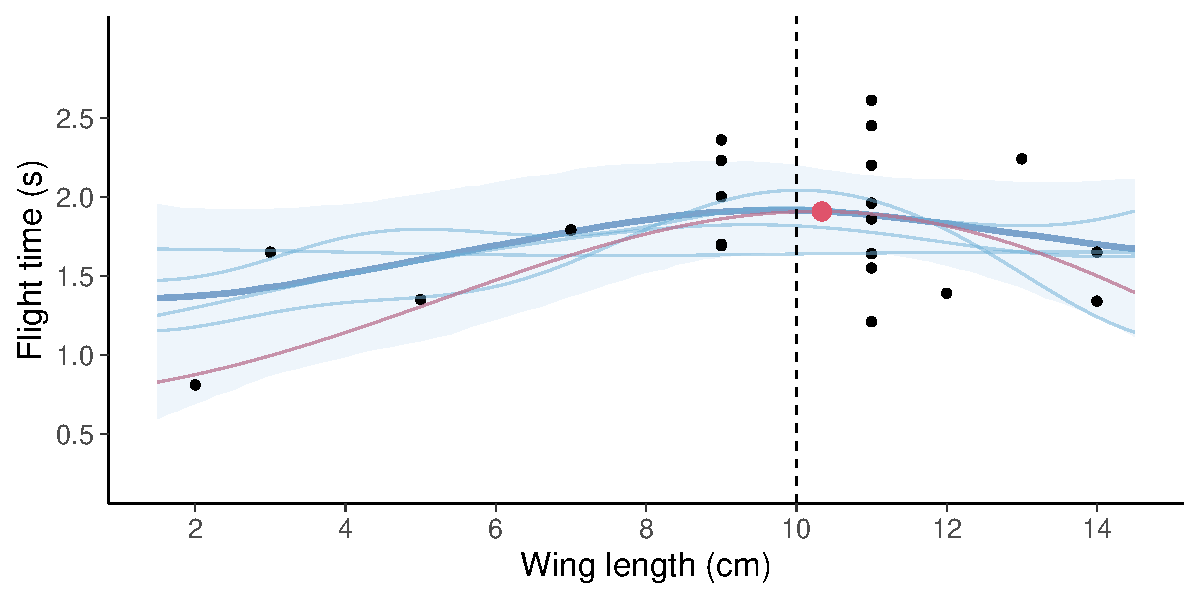
\includegraphics[width=11.5cm]{helicopter_bo_b_17.pdf}}
\only<+>{\hspace{-8mm}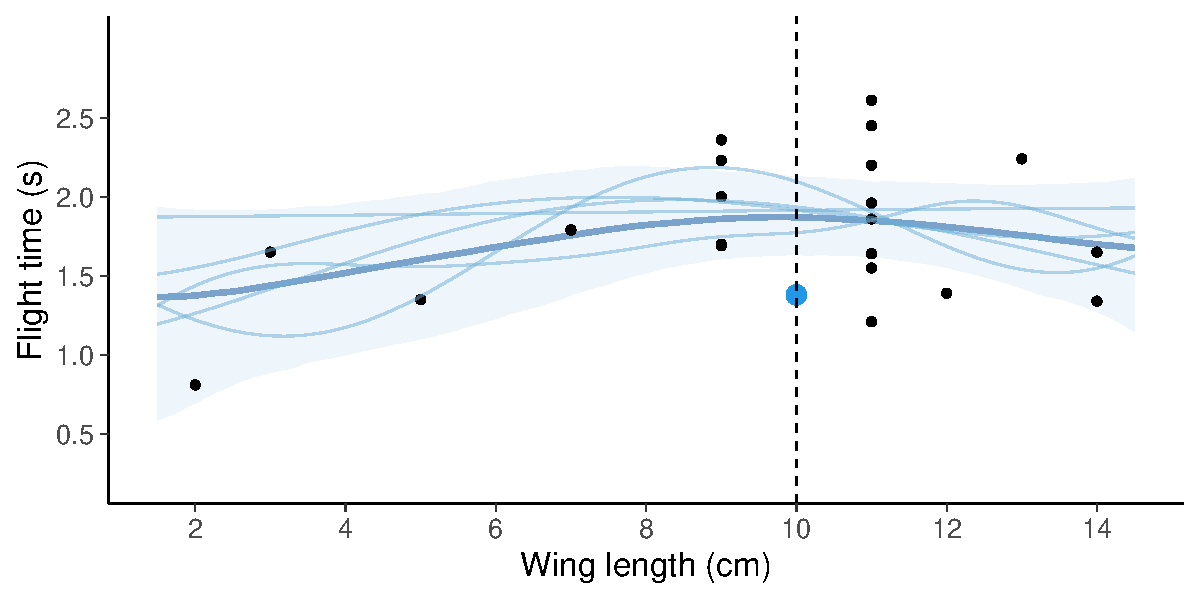
\includegraphics[width=11.5cm]{helicopter_bo_a_18.pdf}}
\only<+>{\hspace{-8mm}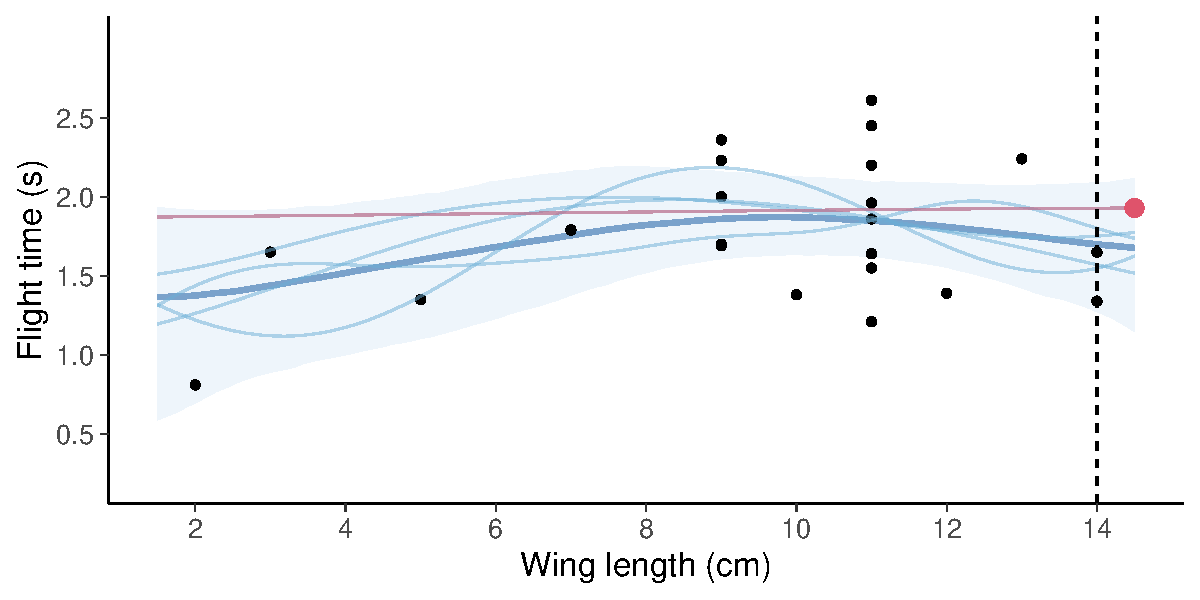
\includegraphics[width=11.5cm]{helicopter_bo_b_18.pdf}}
\only<+>{\hspace{-8mm}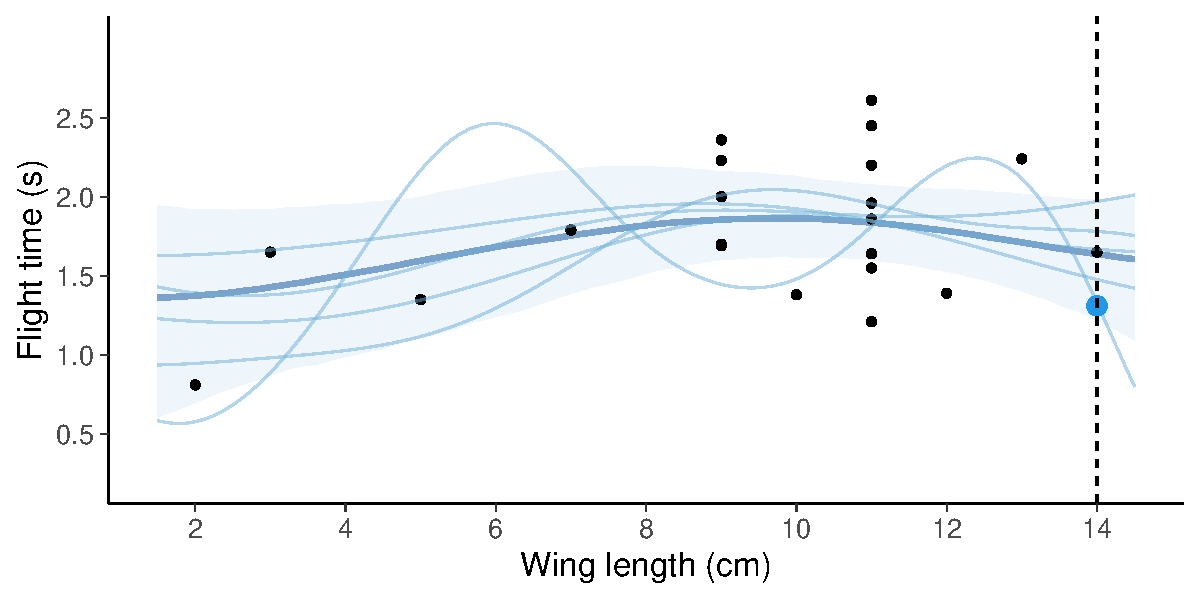
\includegraphics[width=11.5cm]{helicopter_bo_a_19.pdf}}
\only<+>{\hspace{-8mm}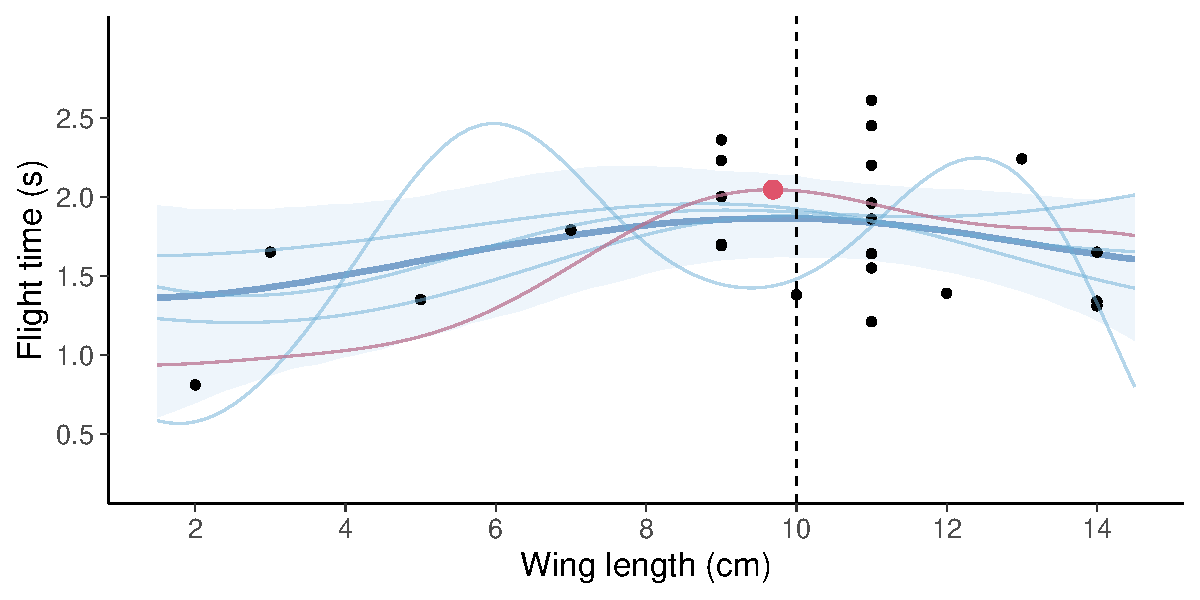
\includegraphics[width=11.5cm]{helicopter_bo_b_19.pdf}}
\only<+>{\hspace{-8mm}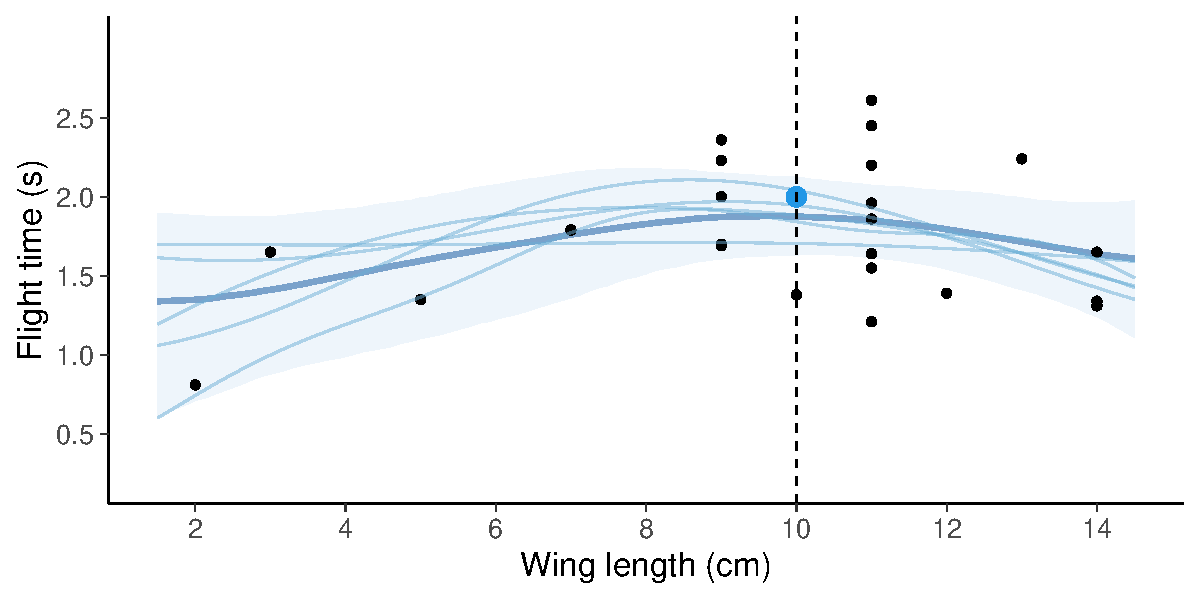
\includegraphics[width=11.5cm]{helicopter_bo_a_20.pdf}}
\only<+>{\hspace{-8mm}\includegraphics[width=11.5cm]{helicopter_bo_b_20.pdf}}
\only<+>{\hspace{-8mm}\includegraphics[width=11.5cm]{helicopter_bo_a_21.pdf}}
\only<+>{\hspace{-8mm}\includegraphics[width=11.5cm]{helicopter_bo_b_21.pdf}}
\only<+>{\hspace{-8mm}\includegraphics[width=11.5cm]{helicopter_bo_a_22.pdf}}
\only<+>{\hspace{-8mm}\includegraphics[width=11.5cm]{helicopter_bo_b_22.pdf}}
\only<+>{\hspace{-8mm}\includegraphics[width=11.5cm]{helicopter_bo_a_23.pdf}}
\only<+>{\hspace{-8mm}\includegraphics[width=11.5cm]{helicopter_bo_b_23.pdf}}
\only<+>{\hspace{-8mm}\includegraphics[width=11.5cm]{helicopter_bo_a_24.pdf}}
\only<+>{\hspace{-8mm}\includegraphics[width=11.5cm]{helicopter_bo_b_24.pdf}}
\only<+>{\hspace{-8mm}\includegraphics[width=11.5cm]{helicopter_bo_a_25.pdf}}
\only<+>{\hspace{-8mm}\includegraphics[width=11.5cm]{helicopter_bo_b_25.pdf}}
\only<+>{\hspace{-8mm}\includegraphics[width=11.5cm]{helicopter_bo_a_26.pdf}}
\only<+>{\hspace{-8mm}\includegraphics[width=11.5cm]{helicopter_bo_b_26.pdf}}
\only<+>{\hspace{-8mm}\includegraphics[width=11.5cm]{helicopter_bo_a_27.pdf}}
\only<+>{\hspace{-8mm}\includegraphics[width=11.5cm]{helicopter_bo_b_27.pdf}}
\only<+>{\hspace{-8mm}\includegraphics[width=11.5cm]{helicopter_bo_a_28.pdf}}
\only<+>{\hspace{-8mm}\includegraphics[width=11.5cm]{helicopter_bo_b_28.pdf}}
\only<+>{\hspace{-8mm}\includegraphics[width=11.5cm]{helicopter_bo_a_29.pdf}}


\end{frame}

\begin{frame}{Bayesian optimization of wing length}

  {\hspace{-8mm}\includegraphics[width=11.5cm]{helicopter_bo_maximizing_density_2.pdf}\\
    \uncover<2->{33 BO obs. post. Wasserstein-1 distance $\approx$ 0.77\\
      33 first obs. post. Wasserstein-1 distance $\approx$ 1.36}\\}
  \uncover<3->{~\\We obtain about 50\% increase in efficiency}
% \only<3>{\hspace{-8mm}\includegraphics[width=11.5cm]{helicopter_bo_maximizing_density.pdf}
%     33 BO obs. post. Wasserstein-1 distance $\approx$ 0.77\\
%     5 first + 28 random obs. post. Wasserstein-1 distance $\approx$ 1.27}
  
\end{frame}  

\begin{frame}{Examples of big Bayesian decision making success stories}

  \begin{list1}
    \item Bayesian optimization of ML algorithms
    \item Bayesian optimization of new medical molecules
    \item Bayesian optimization of new materials
    \item A/B testing
    \item Customer retention / satisfaction
    \item Marketing
  \end{list1}
  
\end{frame}

\end{document}

%%% Local Variables:
%%% mode: latex
%%% TeX-master: t
%%% End:
